\documentclass[english,letterpaper,12pt,oneside,openany]{book}
\usepackage[english]{babel}
\usepackage{babelbib}
\usepackage{etoolbox}
\usepackage{mathtools}
\usepackage{cancel}
\patchcmd\btxselectlanguage{\csname}{\csname TEMPPATCH}{}{} % Para hacer a babelbib funcionar
\usepackage{amstext, amssymb, amsthm, amsmath, amsbsy}
\usepackage{tabularx}
\usepackage[ansinew]{inputenc}
\usepackage[margin=20pt,font=small,labelfont=bf,labelsep=period]{caption}%%Para modificar el formato del texto de los "caption"
\usepackage{graphicx}
\usepackage{url}
\usepackage{listings}%%Para incluir codigo
\usepackage[final]{pdfpages}%%Para incluir archivos en pdf
\usepackage{geometry}
\usepackage{enumerate}
\usepackage{subfig}%%Para incluir subgraficos
\usepackage[pdftex, pdftitle={Finite Element Methods}, pdfauthor={J. Gomez, N. Guarin-Zapata}, pdfsubject={Class Notes}, pdfkeywords={Computational Mechanics, Finite Element Methods}, pdfpagemode=UseOutlines,bookmarks,bookmarksopen,pdfstartview=FitH,colorlinks,linkcolor=blue, urlcolor=black, citecolor=blue]{hyperref} %%Para incluir detalles cucas del pdf
\usepackage[ruled]{algorithm2e}%%Para incluir algoritmos
\usepackage{float}
\usepackage{multirow}
\usepackage{leftidx}
\usepackage{algorithm2e}
%\usepackage{algorithmic}
\usepackage{cite}  %% Para poner bonitas las citas
\usepackage{bookmark} %% Para poder organizar las etiquetas en pdf
\geometry{verbose,letterpaper,tmargin=3cm,bmargin=3cm,lmargin=2cm,rmargin=2cm}
%%%%%%%%%%%%%%%%%%%%%%%%%%%%%%%%%%%%%%%%%%%%%%%%%%%%%%%%%%%%%%%%%%%%%%%%%%%%
%Nuevos Comandos

\setlength{\parskip}{0.5cm}

% Comillas:   ``''

\newcommand{\urlbib}[1]{{\footnotesize{\url{#1}}}} % para incluir urls en las referencias
\newcommand{\fullref}[1]{\ref{#1} de la p\'agina \pageref{#1}}

%%%%%%%%%%%%%%%%%%%%%%%%%%%%%%%%%%%%%%%%%%%%%%%%%%%%%%%%%%%%%%%%%%%%%%%%%%%%
\usepackage{cleveref}
\begin{document}
%%
%\renewcommand{\tablename}{Tabla}
%\renewcommand{\figurename}{Figura}
%\renewcommand{\contentsname}{Table of Contents}
%\renewcommand{\listtablename}{Lista de tablas}
%\renewcommand{\listfigurename}{Lista de figuras}

%%
%%%%%%%%%%%%%%%%%%%%%%%%%%%%%%%%%%%%%%%%%%%%%%%%%%%%%%%%%%%%%%%%%%%%%%%%%%%%
%%%%%%%%%% Portada %%%%%%%%%%
%Portada
%
\begin{center}
\Large{Class Notes: Introduction to the Finite Element Methods}
\large
\\[30mm]
Juan David G\'omez Cata\~no\\
\emph{jgomezc1@eafit.edu.co}
\\[40mm]
Grupo de Investigacion en Mecanica Aplicada
\\
Civil Engineering Department
\\
School of Engineering
\\
Universidad EAFIT
\\
Medell\'in, Colombia
\\
2013
\end{center}
\thispagestyle{empty}

\frontmatter
%%%%%%%%%%%%%%%%%%%%%%%%%%%%%%%%%%%%%%%%%%%%%%%%%%%%%%%%%%%%%%%%%%%%%%%%%%%%
% Tabla de contenido
\pdfbookmark[0]{Tabla de contenido}{}
\tableofcontents


\mainmatter
%%%%%%%%%%%%%%%%%%%%%%%%%%%%%%%%%%%%%%%%%%%%%%%%%%%%%%%%%%%%%%%%%%%%%%%%%%%%
%%%%%%%%%% Introduccion %%%%%%%%%%
%Seccion "Resumen"
%

\cleardoublepage \phantomsection
\addcontentsline{toc}{chapter}{Summary}
\chapter*{Summary}

\vspace{-1cm}

Class Notes for the Course Introduction to the Finite Element Methods


\textbf{Palabras clave: } Computational Mechanics, Finite Element Methods.

%Chapter "Introduction"
%
\chapter{Introduction}

In an introductory graduate course in the Finite Element Method (FEM), the purpose is to develop a basic understanding of the discrete or numerical strategy of Finite Element-(FE) Algorithms when a closed form solution to a Boundary Value Problem (BVP) is not possible due to complexities existing probably: in the boundary conditions, material behavior or in the kinematic description used in the model. In such a course, in order to master and identify the main mathematical and algorithmic aspects of the method at the beginners level, the studied problem is kept lineal. In this sense 4 key aspects make the core of the introductory course (at least for the case of the linearized theory of elasticity boundary value problem):

\begin{itemize}

\item Formulation and identification of the strong form of the Boundary Value Problem (BVP) where the continuum mechanics governing equations are revisited and particularized to the case of linear elastic material behavior. The BVP is completed by identifying the correct prescription of boundary conditions for a well posed mathematical problem.

\item Formulation and identification of the weak form of the BVP where the governing equations and natural boundary conditions representing equilibrium at the material point level are replaced by an equivalent but weaker form of equilibrium now valid at the global level.  In the case of a Continuum Mechanics problem this so-called weak form can be shown to be equivalent to the principle of virtual power and lends itself for the partition of the problem into sub-domains or finite size elements.

\item Introduction of the idea of discretization dividing the problem into subdomains and using interpolation theory within each subdomain-In the context of the FE method this is the subject of shape functions. Once the computational specimen has been divided into subdomains (or a mesh of finite elements) the selected primary variable is approximated within each element via interpolation of the known response at selected predefined points or nodes.

\item Computational aspects grouped also into 5 points:
	\begin{itemize}
	\item Formulation of elemental matrices in the physical space.
	\item Formulation of elemental matrices in the natural domain-Isoparametric transformation.
	\item Numerical integration: Gauss quadrature.
	\item Assembly of system matrices and imposition of boundary conditions.
	\item Solution of the discrete equilibrium statement and calculation of elemental results.
	\end{itemize}
\end{itemize}

These 4 key points are perfectly well documented in numerous nicely written textbooks and it could be argued that is not even worth to register for an introductory course since a moderately dedicated student can accomplish the task via self-study. Unfortunately, linearity is scarce--although useful to grasp the basic understanding of the problem--and the real world is full of non-linear behavior and understanding the needed algorithms can be easily justified. In this \todo{Check name of the ```course".}\textcolor{red}{Advanced Finite Element Methods course} the goal is then to understand the basic aspects of non-linear finite element analysis.  Like in the linear case there is also a vast amount of literature for the non-linear problem.  However, in the non-linear case the kinematic problem itself may take different routes leading to a wide variety of FEM formulations that will difficult a self-study strategy.  Considering the above this brief set of class notes is intended as a guide for self-study and more important represents a help towards the implementation of the algorithm for the consideration of Material and Geometric Non-linearities in Solids.

The basic reference is Professor Bathe's textbook \cite{book:bathe} but we will also follow closely ABAQUS Theory Manual \cite{abaqus_theory}. ABAQUS is a multi-physics oriented commercially available finite element analysis tool. Its strength resides in the effective non-linear algorithms and on the capability of taking user subroutines written in Fortran or in \CPP.  The possibility of implementing user subroutines makes it a very powerful research tool.  In the particular case of a stress/displacement analysis problem with non-linearities these are considered through the kinematics contribution or through the material contribution.  In the first case the non-linear behavior must be considered at the element level while in the second it corresponds to the response of a material point which in the context of the FEM algorithm corresponds to an integration point. In ABAQUS those two sources of non-linearity can be independently controlled by the user via user subroutines UEL and UMAT.  In both cases the non-linearity is primarily solved by the classical Newton-Raphson scheme and that will be the approached followed herein.  Although the notes are mainly written for an advanced course the specific problem of a linear solid usually studied in the introductory course can be derived like a particular case of the most general non-linear algorithm.

The current set of Class Notes is organized as follows.  First and since we will be dealing with history dependent non-linear problems the most powerful (at least when it works) solution algorithm, namely the Newton-Raphson iteration is studied.  The technique is first illustrated for the simple 1D-case and then generalized into the multi-degree of freedom system.  In both cases pseudo-codes will be presented preparing the way for the Finite Element Algorithm.  The presentation however is not exhaustive in mathematical terms and the reader is referred to excellent treatments like Burden \cite{book:burden2011} and Press et al. \cite{book:numerical_recipes} for the mathematical aspects of the Newton method.

In the next section the briefly introduced Newton-Raphson technique is contextualized to the case of a system of equations representing equilibrium between internal and external forces as typically found in a finite element model.  Moreover, the non-linearities come into play through a dependence of the internal forces into displacements.  At this stage the details of the formulation of the finite element equations via discretization into nodal variables is not presented but emphasis is laid down into the solution algorithm.  Interest is then given to the particular form taken by the Newton-Raphson algorithm into the commercial finite element code ABAQUS.  That code can be used as a powerful non-linear equation solver where the coefficient matrix and the excitation can be directly controlled by the user.  Moreover the solver can be used into a multi-physics context in terms of generalized forces and fluxes.  In the particular case of the stress analysis finite element method the user can control the elemental contribution to the coefficient matrix and the contribution of each material point to obtain that element contribution.  This is achieved through the so-called user subroutines UEL  for element and UMAT  for material.  Having introduced the Newton-Raphson method the notes concentrate next on general discretization aspects starting from the physical strong form of the equations in the deformed configuration and passing to an arbitrary weak form in the reference configuration.  The resulting algorithm is therefore a Total Lagrangian (TL) method.  Once the general equations are introduced a particular work conjugate stress-strain pair is chosen and the discrete equations, including kinematic interpolators, are described.

\section*{Notation}
In a non-linear algorithm the bookkeeping is involved since we have to simultaneously record 4 different fields as follows:
\begin{itemize}
	\item The physical fields in terms of tensorial descriptions.
	\item The time field since the problem is solved incrementally 	and time may appear as an artificial chronological variable 	or as a real quantity in a dynamic problem.
	\item The interpolation field.  Since all the involved variables will be interpolated we will need to keep track of the way this interpolation is being performed.
	\item The iterations field needed in the solution of the non-linear problem.
\end{itemize}
In order to keep this bookkeeping simple we use the following indicial notation with subscripts and superscripts

\begin{figure}[h]
\centering
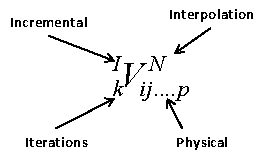
\includegraphics[width=4cm]{img/figure1_1.pdf}
\caption{General notation to study non-linear finite element problems}
\label{fig:notation}
\end{figure}

\todo{Review notation.}Capital superscripts will be reserved for the incremental time description and for the interpolation scheme.  For instance an expression like   refers to the time instant   while   refers to . Similarly a variable   refers to interpolation over the node. Left and right subscripts will be used to make reference to the iteration being performed and the order of the tensor variable.  For instance   refers to a second order tensor corresponding to the iteration.
%
\graphicspath{ {./img/TheFEM/} }
\chapter{The Finite Element Method}
\section{Boundary value problems}
In this section we will define a general initial boundary value problem (I-BVP). In the first part we will introduce the differential formulation given in terms of a set of governing equations and properly specified boundary conditions. The resulting equations are obtained after using a generalized balance law. Following this classical and well known approach we formally re-state these equations in the so-called strong form. Subsequently we re-write and prove an equivalent form of the balance law in the form of an integral representation highly friendly for a numerical solution. Since in the integral description of the problem the order of the derivatives in the field functions decreases by one, the resulting statement is called a weak formulation. 
%%
\subsection{Differential formulation-Generalized balance law}
Let $ds$ be a differential surface element; $dV$ a differential volume element; $u(\vec x,t)$ a scalar (or vector) function of space and time.
The flux or rate of flow of the quantity $u(\vec x,t)$ through $ds$ at time $t$ is defined like;
\[p(\vec x)\vec \nabla u \cdot \hat nds\]

where $p(\vec x)$ is a positive function, assumed known and time independent. Similarly, the time rate of change of $u(\vec x,t)$ in an element $dV$ is given by;

\[\rho (\vec x)\frac{{\partial u}}{{\partial t}}dV\]

where once again $\rho (\vec x)$ is a known, given, time independent positive function. Additional effects occurring in the element $dV$ at the time time can be expressed like;

\[H(\vec x,t)dV \equiv  - q(\vec x)u(\vec x,t) + \hat F(\vec x,t)\]

where $\hat F(\vec x,t) = \rho (\vec x)F(\vec x,t)$. In the above the term $qu$ represent internal effects due to changes proportional to $u$ while $\hat F(\vec x,t)$ are other external influences in the medium.

Balancing the internal and external changes yields;

\[\int\limits_V {\rho (\vec x)\frac{{\partial u}}{{\partial t}}dV = \int\limits_S {p(\vec x)\vec \nabla u \cdot \hat nds} }  + \int\limits_V {H(\vec x,t)dV} \]

or equivalently;

\[\int\limits_V {\rho (\vec x)\frac{{\partial u}}{{\partial t}}dV = \int\limits_S {p(\vec x)\vec \nabla u \cdot \hat nds} }  - \int\limits_V {q(\vec x)u(\vec x,t)dV}  + \int\limits_V {\rho (\vec x)F(\vec x,t)dV} \]

using the divergence theorem as

\[\int\limits_S {p(\vec x)\vec \nabla u \cdot \hat nds}  = \int\limits_V {\vec \nabla  \cdot \left( {p\vec \nabla u} \right)dV} \]

yields after substitution;

\[\int\limits_V {\left[ {\rho (\vec x)\frac{{\partial u}}{{\partial t}} - \vec \nabla  \cdot \left( {p(\vec x)\vec \nabla u} \right) + q(\vec x)u(\vec x,t) - \rho (\vec x)F(\vec x,t)} \right]dV}  = 0\]

Assuming a continuous integrand, the arbitrariness of $V$ implies;

\[
\rho (\vec x)\frac{{\partial u}}{{\partial t}} - \vec \nabla  \cdot \left( {p(\vec x)\vec \nabla u} \right) + q(\vec x)u(\vec x,t) - \rho (\vec x)F(\vec x,t) = 0
\]

Letting;

\[L() \equiv  - \vec \nabla  \cdot \left( {p(\vec x)\vec \nabla } \right) + q(\vec x)\]

the generalized set of partial differential equations can be written like;

\begin{equation}
\rho (\vec x)\frac{{\partial u(\vec x,t)}}{{\partial t}} + Lu(\vec x,t) = \rho (\vec x)F(\vec x,t)
\label{GenPDE}
\end{equation}

\begin{itemize}
\item Hyperbolic;
\[\rho (\vec x)\frac{{{\partial ^2}u(\vec x,t)}}{{\partial {t^2}}} + Lu(\vec x,t) = 0\]

\item Parabolic;
\[\rho (\vec x)\frac{{\partial u(\vec x,t)}}{{\partial t}} + Lu(\vec x,t) = 0\]

\item Elliptic;
\[Lu(\vec x,t) = \rho (\vec x)F(\vec x,t)\]
 
\end{itemize}

It can be shown that $L()$ satisfies symmetry;

\[\int\limits_V {L(u)vdV = } \int\limits_V {L(v)u} dV\]

and positive definiteness;

\[\int\limits_V {L(u)udV}  > 0\]

\subsection*{Strong form}
Given $\rho (\vec x)$,$q(\vec x)$, $p(\vec x)$, $F(\vec x,t)$ and $\bar u$ find $u(\vec x , t):V \to \mathbb{R}$ such:
\[
\rho (\vec x)\frac{{\partial u}}{{\partial t}} - \vec \nabla  \cdot \left[ {p(\vec x)\vec \nabla u} \right] + q(\vec x)u(\vec x,t) - \rho (\vec x)F(\vec x,t) = 0
 \quad \forall \vec x \in V \]
 


and

\[u = \bar u \quad for \quad {\vec x} \quad in \quad S_u\]

\[p(\vec x){u_{,i}}{{\hat n}_i} = B(\vec x,t) \quad for \quad {\vec x} \quad in \quad S_t\].

In the FEM we will look for approximate solutions to $u$ subject to the following conditions:

\[u = \bar u \quad for \quad {\vec x} \quad in \quad S_u\] (Essential boundary conditions)

and

\[{\int\limits_S {\left( {\frac{{\partial u}}{{\partial {x_j}}}} \right)} ^2}dS < \infty \] which corresponds to the functions being square integrable. This is space is denoted by $\mathbb{H}$ .

The space of functions satisfying the above two conditions will be denoted by $\zeta $ and termed the space of trial functions, formally defined like:

\[\zeta  = \left\{ {u \mid u \in \mathbb{H},u = \bar u \quad for \quad \vec x \quad in \quad S_u} \right\}\]

On the other hand, in order to validate (or test) the correctness of the approximated or proposed trial functions $u$ it is also necessary to introduce test functions $w$ which are arbitrary except that they satisfy the following conditions:

\[w = 0 \quad for \quad {\vec x} \quad in \quad S_u\] 

and

\[{\int\limits_S {\left( {\frac{{\partial w}}{{\partial {x_j}}}} \right)} ^2}dS < \infty \] which corresponds to the functions being square integrable. The space of functions satisfying the above two conditions will be denoted by $\pounds$ and termed the space of test functions, formally defined like:

\[\pounds  = \left\{ {w \mid u \in \mathbb{H},w = 0 \quad for \quad \vec x \quad in \quad S_u} \right\}\]

\subsection*{Weak form}
Given $\rho (\vec x)$,$q(\vec x)$, $p(\vec x)$, $F(\vec x,t)$ and $\bar u$ find $u(\vec x , t):V \to \mathbb{R}$ and $\forall w \quad \in \quad \pounds $ such:

\[\int\limits_V {[p(\vec x)u{,_i}]} {w_{,i}}dV - \int\limits_{{S_t}} {B(\vec x,t)wdS}  + \int\limits_V {q(\vec x)u(\vec x,t)wdV}  + \int\limits_V {\rho (\vec x)\frac{{\partial u}}{{\partial t}}wdV - \int\limits_V {\rho (\vec x)F(\vec x,t)wdV = 0} } \]

and

\[u = \bar u \quad for \quad {\vec x} \quad in \quad S_u\]

\subsection*{Equivalence between the strong and weak forms}

\begin{multline}
- \int\limits_V {{{[p(\vec x)u{,_i}]}_{,i}}wdV}  + \int\limits_{{S_t}} {[p(\vec x)u{,_i}]} {{\hat n}_i}wdS - \int\limits_{{S_t}} {B(\vec x,t)wdS} \\
  + \int\limits_V {q(\vec x)u(\vec x,t)wdV}  + \int\limits_V {\rho (\vec x)\frac{{\partial u}}{{\partial t}}wdV - \int\limits_V {\rho (\vec x)F(\vec x,t)wdV = 0} }
\end{multline}

Grouping together common terms yields;

\[\int\limits_V {\left\{ {\rho (\vec x)\frac{{\partial u}}{{\partial t}} - {{[p(\vec x)u{,_i}]}_{,i}} + q(\vec x)u(\vec x,t) - \rho (\vec x)F(\vec x,t)} \right\}} wdV + \int\limits_{{S_t}} {\left\{ {[p(\vec x)u{,_i}]{{\hat n}_i} - B(\vec x,t)} \right\}} wdS = 0\]

from which;

\[\rho (\vec x)\frac{{\partial u}}{{\partial t}} - {[p(\vec x)u{,_i}]_{,i}} + q(\vec x)u(\vec x,t) - \rho (\vec x)F(\vec x,t) = 0\]

and

\[p(\vec x){u_{,i}}{{\hat n}_i} = B(\vec x,t)  \quad for \quad {\vec x} \quad in \quad S_t\]










\section{Brief review of the linearized theory of elasticity model}
Here we present a brief description of the boundary value problem governing the response of an elastic body. For a full discussion of the model and its mathematical aspects the reader is referred to \cite{shames1997elastic}.

The governing equations (in terms of stresses) stem from the principle of conservation of linear momentum and conservation of moment of linear momentum. The former leads to a set of 3 partial differential equations in the components of the stress tensor while the latter leads to the symmetries in the stress tensor.

\begin{equation} \label{eq:pde}
\begin{aligned}
&\sigma_{ij,j} + {f_i} = \rho\ddot{u}_i \quad \forall\ \vb{x} \in V,\, t \in \mathbb{R}^{+}\\
&\sigma_{ij}=\sigma _{ji}.
\end{aligned} 
\end{equation}

In \cref{eq:pde} $\sigma_{ij}$ is the stress tensor; $f_i$ is the vector of body forces; and $u_i$ is the displacements vector.

Denoting the tractions vector associated with a surface with normal direction $\hat{n}_{j}$ by $t_i^{\hat n}$ we have the complete BVP as follows:

\begin{equation} \label{eq:bcs}
t_i^{\hat n} = \sigma_{ij} \hat{n}_{j} \quad \forall \in \vb{x} \in S.
\end{equation}

\Cref{eq:pde} correspond to 6 equations with 12 unknowns (the 9 components of the stress tensor and the 3 components of the displacements vector ) and the system is undetermined. In order to have a solvable BVP we must introduce kinematic strain-displacement relations and a stress-strain law. In the case of infinitesimal theory of elasticity the strain-displacement relation is given by:

\begin{equation}\label{eq:kin}
\varepsilon_{ij} = \frac{1}{2}(u_{i,j} + u_{j,i})
\end{equation}

where the term $\epsilon_{ij}$ is the symmetric component of the displacements gradient tensor. The components of the strain tensor describe the distortions and changes in magnitude (volumetric changes) of the material point in the continuum model. Now the simplest stress-strain (constitutive) relationship is given by Hooke's law\footnote{Despite the name of \emph{law} used, this relation is not always valid, but is a good approximation for small strains.}

\begin{equation} \label{eq:Hooke}
\sigma_{ij} = 2\mu \varepsilon_{ij} + \lambda \varepsilon_{kk}\delta_{ij} \enspace .
\end{equation}

where $\mu$ and $\lambda$ are material constants. The problem involves now a total of 18 equations and 18 unknowns can be solved if subjected to properly specified boundary conditions.

\subsection*{Displacement formulation}
Substituting \cref{eq:kin} in \cref{eq:Hooke} and the result in \cref{eq:pde} yields after some manipulation:

\begin{equation} \label{eq:navier}
(\lambda  + \mu)u_{j,ij} + \mu u_{i,jj} + {f_i} = \rho \ddot{u}_i \quad \forall \vb{x} \in V,\, t \in \mathbb{R}^{+}.
\end{equation}

Since \cref{eq:navier} ( simultaneously describing equilibrium, kinematic relations and constitutive response) is a second order equation governing the displacement field possible boundary conditions are in terms of the variable itself or its first oder derivatives. For a well-possed problem the following is a set of valid boundary conditions: 

\begin{equation} \label{eq:Wellbcs}
\begin{split}
&t_i^{\hat n} = \sigma _{ij} \hat n_{ij} \quad \forall\ \vb{x} \in S_t\\
& {u_i} = \bar{u}_i \quad \forall \vb x \in S_u
\end{split}
\end{equation}

and where ${S_t} \cup {S_u} = S$ and ${S_t} \cap {S_u} = \emptyset $. 


In the particular case in which $u_i$ is not a function of time, we obtain the static version of the BVP, i.e,
\begin{equation}
\begin{split}
&\left(\lambda  + \mu \right)u_{j,ij} + \mu u_{i,jj} + {f_i} = 0 \quad \forall \vb{x} \in V \\
&t_i^{\hat n} = \sigma _{ij} \hat n_{ij} \quad \forall\ \vb{x} \in S_t\\
& {u_i} = \bar{u}_i \quad \forall \vb x \in S_u
\end{split}
\end{equation}

Notice that the tractions BC 
\[t_i^{\hat n} = \mu (u_{i,j} + u_{j,i}) \hat{n}_j + \lambda u_{k,k} \delta_{ij}\hat{n}_j \enspace ,\]

actually involves first order displacements derivative and as such it is a Neumann boundary condition on $u_i$.
%

\subsection{Equivalence between strong and weak forms}
\subsubsection{Strong form}
The strong form corresponds to the differential formulation of the problem, it is denoted by $\{ S \}$ and it reads:

Given $f_i$, $t_i^{\hat n}$ and ${\bar u_i}$ find ${u_i}:V \to \mathbb{R}$ such:
%
\begin{equation} \label{eq:navier_2}
\begin{split}
&(\lambda  + \mu)u_{j,ij} + \mu u_{i,jj} + f_i = 0 \quad \forall \vb{x} \in V \\
&t_i^{\hat n} = \sigma _{ij} \hat{n}_{ij} \quad \forall \vb{x} \in S_t\\
&u_i = \bar{u}_i \quad \forall \vb{x} \in S_u
\end{split}
\end{equation}

In \cref{eq:navier_2} the boundary conditions specified by the traction vector $t_i^{\hat n}$ correspond to the natural boundary conditions, while those specified in terms of the displacements vector $\bar u_i$ represent the essential boundary conditions.

\begin{itemize}
\item We are interested in developing methods to obtain approximate solutions to $\{S\}$.
\item The FEM is formulated starting from a statement equivalent to $\{ S \}$ in which we use trial functions until certain prescribed conditions are met.
\item We will look for solutions $u_i$ subject to the following conditions:
\begin{align*}
&u_i = \bar u_i \qquad \text{in} \qquad S_u\\
&\intL_S \left(\pdv{u_i}{x_j} \right)^2 dS < \infty
\end{align*}

\end{itemize}

The first condition corresponds to the satisfaction of the essential boundary condition, while the second corresponds to the functions being square integrable. The space of functions satisfying the above two conditions is denoted by $\varsigma$ and formally defined like
%
\[\varsigma = \left\{u_i\left| {u_i} \in H, {u_i} = \bar{u}_i \in S_u \right. \right\} \enspace .\]
%
On the other hand, in order to validate the introduced trial functions we also need testing functions $w_i$ also called in the FEM literature weighting or distribution functions. These functions are arbitrary apart from having to satisfy the following conditions:
%
\begin{align*}
&w_i = 0 \quad in \quad {S_u}\\
&\intL_S \left(\pdv{w_i}{x_j}\right)^2 dS < \infty
\end{align*}
%
In what follows we formally denote the space of these functions by $V$ and define it like
%
\[V = \left\{ w_i\left| w_i \in H, u_i = w_i=0 \in S_u \right. \right\} \enspace .\]

\subsubsection{Weak form}
Here we will show that the equilibrium statement represented in the differential formulation can be described in alternative forms. In such description the continuity requirement for the trial functions is weaker than in the strong form leading to the term "weak" statement. Here this alternative representation will be denoted like $\{W\}$ and it reads;

Given $f_i$, $t_i^{\hat n}$ and ${\bar u_i}$ find ${u_i}:V \to \mathbb{R}$ and $\forall {w_i} \in V$ such:

\[\intL_V \sigma _{ij} w_{i,j}\, dV - \intL_V f_i w_i\, dV  - \intL_{S_t} t_i^{\hat n} w_i\, dS = 0\]

\subsubsection*{Proof 1:}
Let $u_i \in \varsigma $ be a solution to $\{S\}$ and let $w_i \in V $. Forming the inner product of the equilibrium statement given in \cref{eq:pde} with $w_i$ and forcing the integral over the domain to be zero we have
%
\[\intL_V (\sigma_{ij,j} + f_i ){w_i}\, dV = 0 \enspace ,\]
%
expanding the terms in the integrand and integrating by parts the first term on the left we have
%
\[\intL_V \sigma _{ij,j} w_i\, dV + \intL_V f_i w_i\, dV = 0 \enspace .\]
\[ - \intL_V w_{i,j} \sigma _{ij}\, dV  + \intL_S \sigma _{ij} \hat{n}_j w_i\, dS  + \intL\limits_V w_i f_i\, dV = 0 \]

since $w_i \in V$ it follows that $w_i = 0$ in $S_u$ from which

\begin{equation}\label{weak}
\intL_V \sigma _{ij} w_{i,j}\, dV - \intL_V f_i w_i\, dV  - \intL_{S_t} t_i^{\hat n} w_i\, dS = 0
\end{equation}

Now, considering that $u_i$ is solution of the strong form $\{S\}$ it must satisfy $u_i = \bar u_{i} \quad \in \quad S_u$ and as a result $u_i \in \varsigma$. On the other hand, since $u_i$ satisfies \cref{weak} $\forall {w_i} \in V$ we have that $u_i$ satisfies the definition of weak solution specified in $\{ W \}$.

\subsubsection*{Proof 2:}
Let $u_i$ be a solution of $\{W\}$ and thus $u_i \in \varsigma$ which means that
\[u_i = \bar u_{i} \quad \in \quad S_u\]
and that it satisfies
\[\intL_V \sigma _{ij} w_{i,j}\, dV - \intL_V f_i w_i\, dV - \intL_{S_t} t_i^n w_i\, dS = 0 \enspace ,\]
integrating by parts,
\[-\intL_V \sigma_{ij,j} w_idV + \intL_S \sigma_{ij} n_j w_i dS  - \intL_V f_i w_i dV - \intL_{S_t} {t_i^n} w_i dS = 0\]

Since ${w_i} \in V$ we have that ${w_i}=0$ in $S_u$ and therefore
\[\intL_V w_i(\sigma_{ij,j} + f_i)dV + \intL_{S_t} w_i( \sigma_{ij} n_j - t_i^n )dS = 0 \]
from which
\begin{equation} \label{equil_2}
\begin{split}
&\sigma_{ij,j} + f_i = 0 \quad \vb{x} \in V \\
&t_i^n = \sigma_{ij} n_j \quad \forall \vb{x} \in S_t\\
&{u_i} = \bar{u}_i \quad \forall \vb{x} \in S_u
\end{split}
\end{equation}

which is once again the strong form of the problem given in \cref{eq:pde}.

\subsection*{Simple wedge under self-equilibrated loads}
Consider the double wedge of side $\ell$ and internal angle $2 \phi$ shown in \cref{fig:WEDGE}. It is assumed to be contained in the $X-Y$ plane, with loading conditions satisfying a plane strain (or plane stress) idealization. The material is elastic with Lame constants $\lambda$ and $\mu$. The wedge is loaded by uniform tractions of intensity $S$ applied over its four faces in such a way that the wedge is self-equilibrated. We wish to find the closed-form elasticity solution for the stress, strain and displacement fields throughout the problem domain.
%
\begin{figure}[H]
\centering
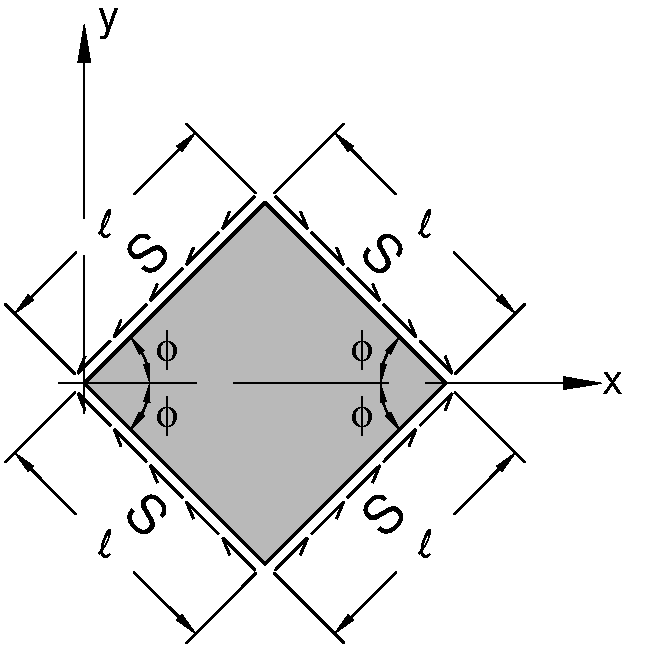
\includegraphics[width=7cm]{wedge.pdf}
\caption{2D Self-equilibrated wedge.}
\label{fig:WEDGE}
\end{figure}

Under plane strain conditions the general 3D stress equilibrium equations (see \cref{eq:pde}) reduce to:
\begin{equation}
\begin{aligned}
&\pdv{\sigma_{xx}}{x}+\pdv{\tau_{xy}}{y}=0\\
&\pdv{\tau_{xy}}{x}+\pdv{\sigma_{yy}}{y}=0
\end{aligned}
\label{eq:equilibrium}
\end{equation}

while the kinematic relation (\cref{eq:kin}) reads

\begin{equation}
\begin{aligned}
\epsilon_{xx}&=\pdv{u}{x}\\
\epsilon_{yy}&=\pdv{v}{y}\\
\gamma_{xy}&=\pdv{u}{y} + \pdv{v}{x}
\end{aligned}
\label{eq:strain}
\end{equation}
where $u$ and $v$ are the horizontal and vertical displacements respectively.

\subsubsection*{Stress field}

The stress field can be obtained by simple inspection from the traction boundary conditions prescribed over the inclined surfaces yielding;

\begin{align*}
\sum F_x &= 0 \longrightarrow - \ell S\cos(\phi)  + \sigma_{xx}\ell \sin(\phi) = 0\\
\sum F_y &= 0 \longrightarrow - \ell S\sin(\phi) - \sigma_{yy}\ell \cos(\phi)=0
\end{align*}

and the following stress solution:

\begin{equation}
\begin{aligned}
\sigma_{xx}& = S \cot(\phi)\\
\sigma_{yy}& = -S\tan(\phi)\\
\tau_{xy}& = 0.
\end{aligned}
\label{eq:solution}
\end{equation}

In \cref{eq:solution} the condition $\tau_{xy}=0$ is due to the symmetries in the problem.

\subsubsection*{Traction boundary conditions}
Let us verify that the above stress solution satisfies the traction BC using the expression:

\[t_i^{\hat n} = \sigma _{ij} \hat n_{ij}.\]

Denoting the outward normals to the inclined surfaces of the wedge by $\hat{n}^1$,  $\hat{n}^2$, $\hat{n}^3$, $\hat{n}^4$ these are given by;
\begin{align*}
\hat{n}^1 &= -\sin(\phi)\hat{e}_{x}+\cos(\phi)\hat{e}_{y}\\
\hat{n}^2 &= -\sin(\phi)\hat{e}_{x}-\cos(\phi)\hat{e}_{y}\\
\hat{n}^3 &= +\sin(\phi)\hat{e}_{x}+\cos(\phi)\hat{e}_{y}\\
\hat{n}^4 &= +\sin(\phi)\hat{e}_{x}-\cos(\phi)\hat{e}_{y} \enspace
\end{align*}

where $\hat{e}_{x}$ and $\hat{e}_{y}$ are the reference unit vectors. Now, the components of the traction vector follow directly like

\[t_{i} = \sigma_{ij}\hat{n}_{j}\]

then over the face with normal $\hat{n}^1$ we have
\begin{align*}
t_{x} &= -S\cos(\phi)\\
t_{y} &= -S\sin(\phi)
\end{align*}
similarly, over the face with normal $\hat{n}^2$
\begin{align*}
t_{x} &= -S\cos(\phi)\\
t_{y} &= +S\sin(\phi)
\end{align*}
over the face with normal $\hat{n}^3$ 
\begin{align*}
t_{x} &= +S\cos(\phi)\\
t_{y} &= -S\sin(\phi)
\end{align*}
and finally, over the face with normal $\hat{n}^4$;
\begin{align*}
t_{x} &= +S\cos(\phi)\\
t_{y} &= +S\sin(\phi) \enspace .
\end{align*}

\subsubsection*{Strain field}
The strain field can be obtained after using the stress solution found in \cref{eq:solution} together with the constitutive law given by \cref{eq:Hooke} which for a plane strain idealization takes the form:

\begin{equation}
\begin{aligned}
{\epsilon _{xx}}& = \frac{1}{E}({\sigma _{xx}} - \nu {\sigma _{yy}}) \\
{\epsilon _{yy}}& = \frac{1}{E}({\sigma _{yy}} - \nu {\sigma _{xx}}) \\
{\gamma _{xy}}& = \frac{{{\tau _{xy}}}}{\mu }
\end{aligned}
\label{eq:cons model}
\end{equation}

which for the particular case yields;


\begin{equation}
\begin{aligned}
\epsilon_{xx}& = +\dfrac{S}{E}\left[\cot(\phi)+\nu \tan(\phi)\right] = +\dfrac{S}{E}K_{1}(\nu , \phi)\\
\epsilon_{yy}& = -\dfrac{S}{E}\left[\tan(\phi)+\nu \cot(\phi)\right] = -\dfrac{S}{E}K_{2}(\nu , \phi)\\
\gamma_{xy}& = 0.
\end{aligned}
\label{eq:strain part}
\end{equation}

\subsubsection*{Displacement field}
The displacement field is obtained after direct integration of the strains after using the fact that:

\[du_i=\epsilon_{ij}dx_j + \omega_{ij}dx_j\]

and the condition $\omega_{xy}=0$ also due to symmetries , as follows:

\begin{align*}
u &= +\dfrac{S}{E} K_{1}(\nu , \phi)x + A\\
v &= -\dfrac{S}{E} K_{2}(\nu , \phi)y + B
\end{align*}

and where $A$ and $B$ are integration constants.

From the condition $u=0$ at $x=\ell\cos(\phi)$ we have that $A=-\dfrac{S}{E} K_{1}(\nu , \phi)\ell\cos(\phi)$ then it follows that
\[u=\dfrac{S}{E} K_{1}(\nu , \phi)(x-\ell\cos(\phi)).\]

Similarly, from the condition $v=0$ at $y=0$ we have that $B=0$ from which
\[v=-\dfrac{S}{E} K_{2}(\nu , \phi)y\]



%%
\subsection{Variational formulation}
In this section we formulate the boundary value problem using the approach of the calculus of variations in which the governing PDEs and boundary conditions are obtained after finding the minimum (or maximum) of a functional according to a variational principle\footnote{According to Wikipedia \cite{wiki:variational_principle}

\begin{quotation}
A variational principle is a scientific principle used within the calculus of variations, which develops general methods for finding functions which minimize or maximize the value of quantities that depend upon those functions. For example, to answer this question: ``What is the shape of a chain suspended at both ends?" we can use the variational principle that the shape must minimize the gravitational potential energy.

According to Cornelius Lanczos, any physical law which can be expressed as a variational principle describes an expression which is self-adjoint. These expressions are also called Hermitian. Such an expression describes an invariant under a Hermitian transformation.
\end{quotation}}.
%%
We will see that the weak form (and therefore also the strong form) can be obtained alternatively through the process of finding extreme values for a functional. We will illustrate this idea for the general case of theory of elasticity and then we will present particular examples.

\subsubsection*{Some vague definitions in the calculus of variations}
In variational calculus a {\bf functional} can be understood as a "function" having as independent variables or arguments a space of vector functions and producing as a result (or dependent variable) a scalar. For instance, in the particular case of the theory of elasticity such a "function" corresponds to the total potential energy functional $\Pi$ given by;

\begin{equation}
\Pi ({u_i}) = \frac{1}{2}\int\limits_V {{\sigma _{ij}}{\varepsilon _{ij}}dV}  - \int\limits_V {{f_i}{u_i}dV}  - \int\limits_S {t_i^{(n)}{u_i}dS}
\label{Potential}
\end{equation}

and where the first term in the L.H.S corresponds to the internal strain energy, while the last two terms are the work done by the external body and traction forces. The above functional has as independent variables the displacement vector and its spatial derivatives. This is indicated by the presence of the displacement vector $u_i$ in the expression $\Pi(u_i)$.

In variational calculus we are interested in finding a function $u_i$ that renders the functional $\Pi$ a maximum or a minimum. In loose terms, the analogous to the differential operator in calculus of functions is now termed the variational operator $\delta$ (i.e., $\delta$ is analogous to $\frac{\partial }{{\partial {x_i}}}$). As such $\delta\Pi$ acts over the function $u_i$ and its derivatives as follows;

\[\delta \Pi  = \frac{{\partial \Pi }}{{\partial {u_i}}}\delta {u_i} + \frac{{\partial \Pi }}{{\partial \left( {\frac{{\partial {u_i}}}{{\partial {x_j}}}} \right)}}\delta \left( {\frac{{\partial {u_i}}}{{\partial {x_j}}}} \right) + ... + \frac{{\partial \Pi }}{{\partial \left( {\frac{{{\partial ^n}{u_i}}}{{\partial {x_j}...\partial {x_k}}}} \right)}}\delta \left( {\frac{{{\partial ^n}{u_i}}}{{\partial {x_j}...\partial {x_k}}}} \right)\].

The following rules apply to the variational operator $\delta$:

\begin{itemize}
\item For functionals $\Pi$ and $\Phi$ it follows that \[\delta (\Pi  + \Phi ) = \delta \Pi  + \delta \Phi \]
\item For functionals $\Pi$ and $\Phi$ it follows that \[\delta (\Pi \Phi ) = \delta \Pi \Phi  + \Pi \delta \Phi \]
\item For a functional $\Pi$ and an integer $n$ it follows that \[\delta ({\Pi ^n}) = n({\Pi ^{n - 1}})\delta \Pi \]
\item For a functional $\Pi$ it follows that \[\delta \int {\Pi dx}  = \int {\delta \Pi dx} \]
\end{itemize}

If the variational operator is applied to the functional $\Pi (u_i)$ it produces functions or variations in $u_i$ which are arbitrary and such $\delta {u_i} \in V$ and $\delta {u_i} = 0$ in $S_u$.

In order to find an extreme function in the calculus of variations we proceed like in differential calculus. Here we compute the first variation of the functional $\delta \Pi$ and solve the variational equation;

\begin{equation}
\delta \Pi  = 0
\label{vareq}
\end{equation}

in the unknown function $u_i$. 

In the particular case of the total potential energy functional $\Pi$ this yields;

\begin{equation}
\int\limits_V {{\sigma _{ij}}\delta {\varepsilon _{ij}}dV}  - \int\limits_V {{f_i}\delta {u_i}dV}  - \int\limits_{{S_t}} {t_i^{(n)}\delta {u_i}dS}  = 0
\label{ClaPVW}
\end{equation}

where we recognize the weak form of the BVP stated previously. It becomes evident that the functions $\delta {u_i}$ in \cref{ClaPVW} play the role of the test functions $w_i$ introduced in the weak form. On the other hand, since we have already shown that the weak and strong forms are equivalent we conclude that having the functional and the essential boundary conditions is equivalent to having the strong form of the problem.


\subsubsection*{Principle of minimum potential energy}
In the theory of elasticity the total potential energy $\Pi$ is the result of adding the elastic strain energy which is stored in the body upon deformation and the potential energy (work) imparted to the body by the applied forces. The principle states that the body is in equilibrium when this total potential energy reaches a minimum. This is equivalent to stating that an equilibrium configuration is attained when an infinitesimal variation from the position of minimum potential energy involves null changes in energy. This implies the variational condition:

\begin{equation}
\delta \Pi  = 0.
\label{vareq2}
\end{equation}

The above principle leads to the so-called principle of virtual displacements stated as follows\footnote{see Bathe pp 156}:
"The equilibrium of the body requires that for any compatible small virtual displacements satisfying the condition of being zero at $S_u$, imposed on the body in its state of equilibrium, the total internal virtual work is equal to the total external virtual work"

\[\int\limits_V {{\sigma _{ij}}\delta {\varepsilon _{ij}}dV}  - \int\limits_V {{f_i}\delta {u_i}dV}  - \int\limits_{{S_t}} {t_i^{(n)}\delta {u_i}dS}  = 0\]

where ${\delta {u_i}}$ are the virtual displacements and ${\delta {\varepsilon _{ij}}}$ are the corresponding virtual strains.

Comparing the virtual work principle with the weak formulation given in \cref{weak} we identify ${\delta {u_i}}$ with the test functions $w_i$. As such the PVW takes the form of a powerful tool to test if a body is in equilibrium for a given solution (represented by the trial functions). In what follows we illustrate the use of the principle through some examples corresponding to problems in Bathe's textbook.

\subsubsection*{Problem 3.15 (In Bathe's book)}
Establish the differential equation of equilibrium of the problem shown and the boundary conditions. Determine whether the differential operator of the problem is symmetric and positive definite and prove your answer.

\begin{figure}[H]
\centering
\includegraphics[width=10cm]{{Bathe3.15}.pdf}
\caption{Rod with varying cross-sectional area. The Young's modulus is E.}
\label{fig:bathe3.15}
\end{figure}


\[\Pi  = \frac{1}{2}\int\limits_0^L {{\sigma _{xx}}{\varepsilon _{xx}}A(x)dx} + \frac{1}{2}ku_0^2 - R{u_L} \]
\[\Pi  = \frac{1}{2}\int\limits_0^L {EA(x){{\left( {\frac{{du}}{{dx}}} \right)}^2}dx + \frac{1}{2}ku_0^2}  - R{u_L}\]

First variation;
\[\delta \Pi  = \int\limits_0^L {EA(x)\frac{{du}}{{dx}}\frac{{d\delta u}}{{dx}}dx + k{u_0}\delta {u_0}}  - R\delta {u_L}\]

Integrating by parts;

\[\delta \Pi  =  - \int\limits_0^L {\frac{d}{{dx}}\left[ {EA(x)\frac{{du}}{{dx}}} \right]\delta udx + \left. {EA(x)\frac{{du}}{{dx}}\delta u} \right]_0^L + k{u_0}\delta {u_0}}  - R\delta {u_L}\]

from which;

\[\frac{d}{{dx}}\left[ {EA(x)\frac{{du}}{{dx}}} \right] = 0\]
\[{\left. {EA(x)\frac{{du}}{{dx}}} \right]_{x = 0}} = k{u_0}\]
\[{\left. {EA(x)\frac{{du}}{{dx}}} \right]_{x = L}} = R\]





\subsubsection*{Problem 4.35-The Hu-Washizu Variational Principle}
Consider the Hu-Washizu functional:
\begin{equation}
\Pi^* = \Pi  - \intL_V \lambda_{ij}^\varepsilon (\varepsilon_{ij} - L_{ijk} u_k)\dd{V}  - \intL_{S_u} \lambda_i^u(u_i^{S_u} - \bar{ u}_i)\dd{S}
\label{eq:Hu}
\end{equation}

where
\begin{itemize}
\item $\Pi$: is the potential energy functional.
\item $L_{ijk}$ is a differential operator such $\varepsilon_{ij} = L_{ijk} u_k$.
\item $S_u$ surface where essential boundary conditions are prescribed.
\item $\lambda_{ij}^\varepsilon $ and $\lambda_i^u$ are Lagrange multipliers.
\end{itemize}

Using the condition $\delta \Pi = 0$ derive for the interior of the body the equilibrium equations;

\[{\sigma _{ij,j}} + {f_i} = 0\]

the strain-displacement relationship;

\[{\varepsilon _{ij}} = {L_{ijk}}{u_k}\]

and the constitutive equation;

\[{\sigma _{ij}} = {C_{ijkl}}{\varepsilon _{kl}}\]

and at the surface of the body the relation between the stress tensor and the applied tractions vector at $S_t$;

\[{t_i} = {\sigma _{ij}}{n_j}\]

the relation between the stress tensor and the unknown tractions vector (or reactions) at $S_u$; 

\[{t_i} = {{\tilde \sigma }_{ij}}{n_j}\]

and the essential boundary condition at $S_u$;

\[{u_i} = {{\tilde u}_i}\]

We want to determine the so-called Euler equations resulting from the condition $\delta \pi^* = 0$. Applying the variational operator we have:
\begin{equation}
\begin{aligned}
\delta \Pi^*& = \delta \Pi  - \intL_V \delta \lambda_{ij}^{\varepsilon}  (\varepsilon_{ij} - L_{ijk} u_k)\dd{V}- \intL_V \lambda_{ij}^\varepsilon (\delta \varepsilon_{ij} - L_{ijk}\delta u_k)\dd{V} \\
&-\intL_V \delta \lambda_i^u (u_i^{S_u} - \bar u_i)\dd{S} - \intL_V \lambda _i^u \delta u_i^{S_u} \dd{S}
\end{aligned}
\end{equation}

\begin{equation}
\begin{aligned}
\delta \Pi^* &= \intL_V C_{ijkl} \varepsilon_{kl} \delta  \varepsilon_{ij}\dd{V} - \intL_{S_t} t_i \delta{u_i} \dd{S}  - \intL_V f_i\delta {u_i}\dd{V} - \intL_V \lambda_{ij}^{\varepsilon} \delta \varepsilon_{ij}\dd{V}  + \intL_V \lambda_{ij}^{\varepsilon} L_{ijk}\delta {u_k}\dd{V}\\
&- \intL_V \delta \lambda_{ij}^{\varepsilon} (\varepsilon_{ij} - L_{ijk} u_k)\dd{V} - \intL_S \delta \lambda_i^u (u_i^{S_u} - \bar {u}_i)dS - \intL_{S_u} \lambda _i^u\delta {u_i}\dd{S} = 0
\end{aligned}
\end{equation}

using

\[\intL_V {(\lambda _{ij}^\varepsilon \delta {u_i}){,_j}dV = } \intL_V {\lambda _{ij}^\varepsilon \delta {u_{i,j}}dV}  + \intL_V {\lambda _{ij,j}^\varepsilon \delta {u_i}dV} \]

in the above we can write

\begin{align*}
\intL_V {\lambda _{ij}^\varepsilon {L_{ijk}}\delta {u_k}dV} & = \intL_V {{{(\lambda _{ij}^\varepsilon \delta {u_i})}_{,j}}dV}  - \intL_V {\lambda _{ij,j}^\varepsilon \delta {u_i}dV}\\
& = \intL_{{S_t}} {\lambda _{ij}^\varepsilon \delta {u_i}{{\hat n}_j}dS}  - \intL_V {\lambda _{ij,j}^\varepsilon \delta {u_i}dV}
\end{align*}

therefore


\begin{align*}
\delta \Pi^* &= \intL_V {({C_{ijkl}}{\varepsilon _{kl}} - \lambda _{ij}^\varepsilon )\delta {\varepsilon _{ij}}dV - \intL_{{S_t}} {{t_i}\delta {u_i}dS}  - \intL_V {{f_i}\delta {u_i}dV + } } \intL_{{S_t}} {\lambda _{ij}^\varepsilon \delta {u_i}{{\hat n}_j}dS}  - \intL_V {\lambda _{ij,j}^\varepsilon \delta {u_i}dV}\\
&- \intL_V {\delta \lambda _{ij}^\varepsilon ({\varepsilon _{ij}} - {L_{ijk}}{u_k})dV}  - \intL_{{S_u}} {\delta \lambda _i^u(u_i^{{S_u}} - {{\bar u}_i})dS}  - \intL_{{S_u}} {\lambda _i^u\delta {u_i}dS}  = 0
\end{align*}


\begin{align*}
&\intL_V {({C_{ijkl}}{\varepsilon _{kl}} - \lambda _{ij}^\varepsilon )\delta {\varepsilon _{ij}}dV
+ \intL_{{S_t}} {(\lambda _{ij}^\varepsilon {{\hat n}_j} - {t_i})\delta {u_i}dS}  - }\\
&\intL_V {(\lambda _{ij,j}^\varepsilon  + {f_i})\delta {u_i}dV}
- \intL_V {({\varepsilon _{ij}} - {L_{ijk}}{u_k})\delta \lambda _{ij}^\varepsilon dV}
- \intL_{{S_u}} {(u_i^{{S_u}} - {{\bar u}_i})\delta \lambda _i^udS}  - \cancel{\intL_{{S_u}} {\lambda _i^u\delta u_i^{{S_u}}dS} = } 0
\end{align*}


Now, imposing the conditions $\delta {\varepsilon _{ij}} \neq 0$, $\delta \lambda _{ij}^\varepsilon  \neq 0$, $\delta {u_i} \neq 0$ in $S_t$, $\delta {u_i} \neq 0$ in $V$ and $\delta \lambda _i^u \neq 0$ in $S_u$ we have
%
\begin{align}
&\lambda _{ij}^\varepsilon  = C_{ijkl} \varepsilon_{kl}\\
&\varepsilon_{ij} = {L_{ijk}}{u_k}\\
t_i &= \lambda_{ij}^\varepsilon \hat{n}_j\\
&\lambda _{ij,j}^\varepsilon  + {f_i} = 0\\
&u_i^{S_u} = \bar{u}_i
\end{align}

\subsection{Weighted residual methods}
In the the following derivations we will assume that the actual solution to the generalized BVP is approximated by the superposition;

\[u(\vec x) = {N^I}(\vec x){u^I}\]

where $I=1,2,...,K$.

Since we are now using an approximation we have the following "unbalanced" condition;

\[Lu(\vec x,t) - \rho (\vec x)F(\vec x,t) = R \ne 0\]

where the term $R$ corresponds to a residual error which is to be distributed throughout the solution domain.



\subsubsection*{Application to the Navier equations}

\[(\lambda  + \mu ){u_{j,ij}} + \mu {u_{i,jj}} + {f_i} = 0\]
\[{L_{ij}} \equiv (\lambda  + \mu )\frac{{{\partial ^2}}}{{\partial {x_i}\partial {x_j}}} + \mu \frac{{{\partial ^2}}}{{\partial {x_k}\partial {x_k}}}{\delta _{ij}}\]
\[{r_i} =  - {f_i}\]
\[{u_i} = N_i^Q{u^Q}\]
\[{L_{ij}}({u_j}) \equiv (\lambda  + \mu ){(N_j^Q{u^Q})_{,ij}} + \mu {(N_j^Q{u^Q})_{,kk}}{\delta _{ij}}\]
\[{L_{ij}}({u_j}) \equiv (\lambda  + \mu )N_{j,ij}^Q{u^Q} + \mu N_{i,kk}^Q{u^Q}\]
\[{L_{ij}}({u_j}) \equiv {L_{ij}}(N_j^Q){u^Q}\]

In the Galerkin scheme we use the trial function as weighting function.

\[{R_i} \equiv {L_{ij}}(N_j^Q){u^Q} + {f_i}\]

and we state



\subsubsection*{Application to the acoustic wave equation}

\section[Discretization of the PVW using FEM]{Discretization of the PVW via the FEM}
\subsection*{A simple spring-mass system}
The simple problem of a spring-mass system considered next resembles most of the algorithmic aspects of a finite element code with the advantage that the problem is already a discrete mechanical system. The problem consists of an assemblage of masses joined by different springs submitted to time varying loads. Each spring plays the role of a finite element and each mass is analogous to a nodal point in a finite element algorithm. For instance the full system may be like the one shown in \cref{fig:bathe}:


\begin{figure}[H]
\centering
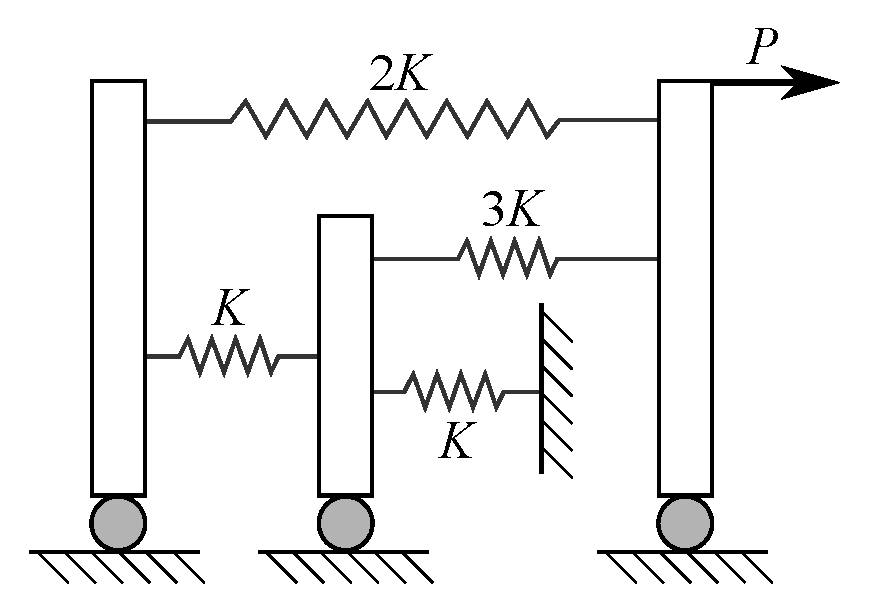
\includegraphics[width=10cm]{spring_system.pdf}
\caption{Typical assemblage of springs and masses.}
\label{fig:bathe}
\end{figure}


Consider a typical spring (finite element) like the one shown in \cref{fig:springel}

\begin{figure}[H]
\centering
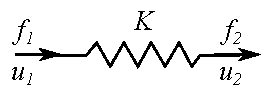
\includegraphics[width=10cm]{springel.pdf}
\caption{Typical spring element.}
\label{fig:springel}
\end{figure}

The relation between the force and the relative displacement can be written like;

\[{f_1} = K({u_1} - {u_2})\]

and from equilibrium we have;

\[{f_1} + {f_2} = 0\]

which yields the following force-displacement relationship for a typical spring element:

\begin{equation}
\left\{ {\begin{array}{*{20}{c}}
{{f_1}}\\
{{f_2}}
\end{array}} \right\} = K\left[ {\begin{array}{*{20}{c}}
{1.0}&{ - 1.0}\\
{ - 1.0}&{1.0}
\end{array}} \right]\left\{ {\begin{array}{*{20}{c}}
{{u_1}}\\
{{u_2}}
\end{array}} \right\}
\label{Kspring}
\end{equation}

On the other hand, the equilibrium equation for a typical mass with displacement $u_j$  (see \cref{fig:dclmass}) and attached to springs $i$ and $i+1$ read;

\begin{equation}
f_2^i + f_1^{i + 1} + {m_j}\frac{{d{V_j}}}{{dt}} = {P_j}.
\label{equilmass}
\end{equation}

which can be written in terms of displacements using \cref{Kspring} like;

\[({K^i} + {K^{i + 1}}){u_j} - {K^i}{u_{j - 1}} - {K^{i + 1}}{u_{j + 1}} + {m_j}\frac{{d{V_j}}}{{dt}} = {P_j}.\]


\begin{figure}[H]
\centering
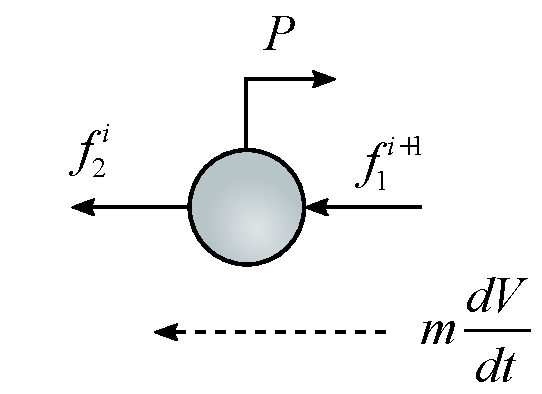
\includegraphics[width=8cm]{dcl_mass.pdf}
\caption{Free body diagram for a typical mass connected to springs $i$ and $i+1$.}
\label{fig:dclmass}
\end{figure}

Considering now the complete system of masses and springs leads to a system of linear equations of the form;

\begin{equation}
\left[ {{K_G}} \right]\left\{ {{U_G}} \right\} + \left[ M \right]\left\{ {{A_G}} \right\} = \left\{ {{F_G}} \right\}.
\label{global}
\end{equation}

where each equation represents the equilibrium of a given mass. The system given by \cref{global} can be solved in the displacements $U_G$. The pseudo-code shown in \cref{springsalg} presents all the steps required to solve the problem in the context of the finite element method. In that code the so-called DME operator is an equation assembly array indicating how each element contributes to the global stiffness and mass matrix.


\begin{algorithm}[H]
 \SetAlgoLined
 \KwData{Problem parameters; NUMNP, NUMEL, NMATP}
 \KwResult{Displacements and spring forces}
 Create $DM$E operator\;
 Assemble $K^G$, $F^G$\;
\While{$j \leq 1, NUMEL$}{
\[
\begin{aligned}
K^G \leftarrow K^G+K^i\\
F^G \leftarrow F^G+F^i\\
\end{aligned}
\]
}
Impose BCs\;
Solve $[K^G]U=F^G$\\
Find internal forces
\caption{Springs Algorithm}
\label{springsalg}
\end{algorithm}


\subsection{Basic elements of interpolation theory}
Let $f(x)$ be a function whose values are known at n discrete points ${x_1, x_2,...,x_n}$. We want to know (interpolate) the value of $f(x)$ at an arbitrary point $x \in \left[ {{x_1},{x_n}} \right]$.

\begin{figure}[h]
\centering
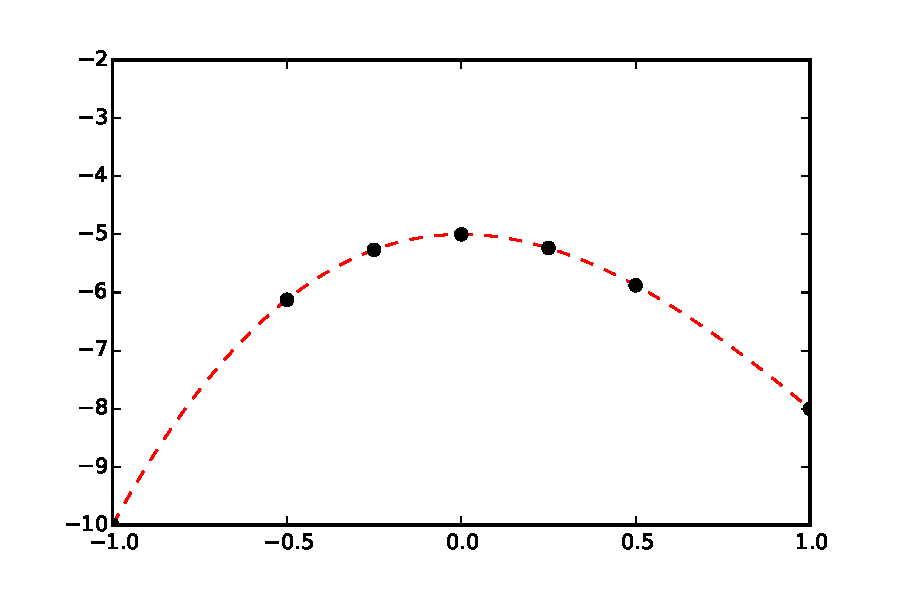
\includegraphics[width=8cm]{img/interpol1.pdf}
\caption{Definition of the natural domain}
\label{fig:interpol1}
\end{figure}

The process of interpolation or computation of the unknown value of $f(x)$ using the known values $\left\{ {{f^1},{f^2},...,{f^n}} \right\}$ involves two steps:

\begin{itemize}
\item[i]  Fitting an interpolating function to the known data points.
\item[ii] Evaluating the function at the arbitrary point.
\end{itemize}

We can (i) use all the n-data points and fit an $(n-1)$-th order polynomial (which is cumbersome and difficult to code) or (ii) split the domain in sub-intervals and use local polynomials within each sub-interval. This last approach involves only a couple of polynomials and it is easy to code, however it may have some continuity issues.

In finite element analysis local interpolation is used in order to proceed systematically. Local interpolation uses a finite number of nearest-neighbors and generates interpolated values $f(x)$ that do not in general have continuous first or higher derivatives.

\begin{figure}[h]
\centering
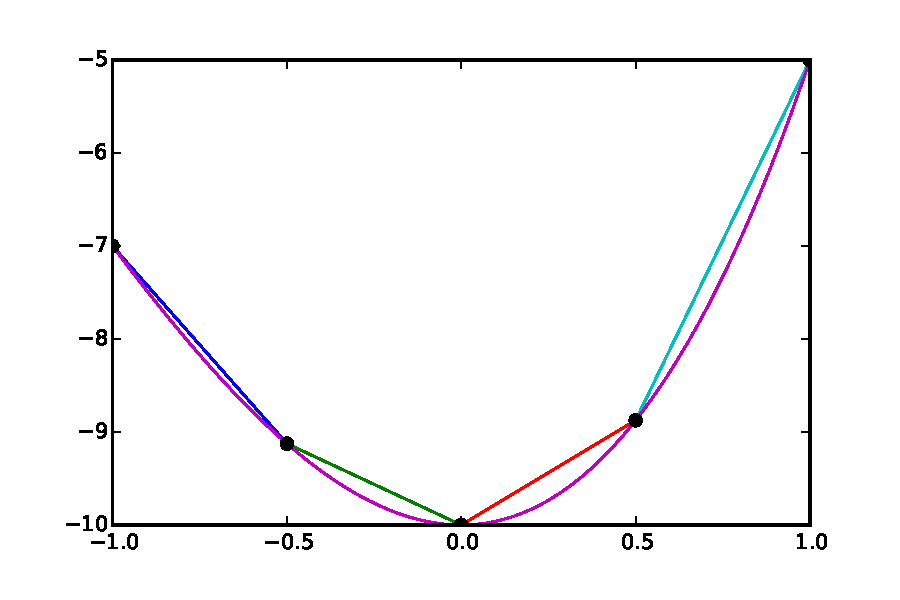
\includegraphics[width=8cm]{img/interpol2.pdf}
\caption{Definition of the natural domain}
\label{fig:interpol2}
\end{figure}

\subsubsection{Lagrange interpolation theorem}
Given a set of n-points $\left\{ {({x^1},{y^1}),...,({x^n},{y^n})} \right\}$ where ${y^n} \equiv f({x^n})$ then: "there exists a unique polynomial $p(x)$ of order at most $(n-1)$ such $p({x^I}) = f({x^I})$ for $I=1,2,...,n$". The polynomial is given by;

\begin{equation}
p({x^I}) = {L^I}(x)f({x^I})
\label{pol}
\end{equation}

for $I=1,2,...,n$ where;

\begin{equation}
{L^I}(x) = \prod\limits_{\scriptstyle J = 1\hfill\atop
\scriptstyle I \ne J\hfill}^n {\frac{{(x - {x^J})}}{{({x^I} - {x^J})}}}
\label{coef}
\end{equation}

and where it should be noticed that

\[{L^I}({x^J}) = {\delta ^{IJ}}.\]

\subsubsection*{Example for n=3}

Consider the domain $[ - 1,1]$ and the data points at ${x^1} =  - 1.0$, ${x^2} =  + 1.0$ and ${x^3} = 0.0$. We have
\[{L^1}(x) = \frac{{\left( {x - {x^2}} \right)\left( {x - {x^3}} \right)}}{{\left( {{x^1} - {x^2}} \right)\left( {{x^1} - {x^3}} \right)}} \equiv  - \frac{1}{2}\left( {1 - x} \right)x\]
\[{L^2}(x) = \frac{{\left( {x - {x^1}} \right)\left( {x - {x^3}} \right)}}{{\left( {{x^2} - {x^1}} \right)\left( {{x^2} - {x^3}} \right)}} \equiv  + \frac{1}{2}\left( {1 + x} \right)x\]
and
\[{L^3}(x) = \frac{{\left( {x - {x^1}} \right)\left( {x - {x^2}} \right)}}{{\left( {{x^3} - {x^1}} \right)\left( {{x^3} - {x^2}} \right)}} \equiv 1 - {x^2}.\]

The resulting interpolating polynomials ${L^I}(x)$ and the interpolating function  are shown in \cref{fig:pols} below:

\begin{figure}[H]
\centering
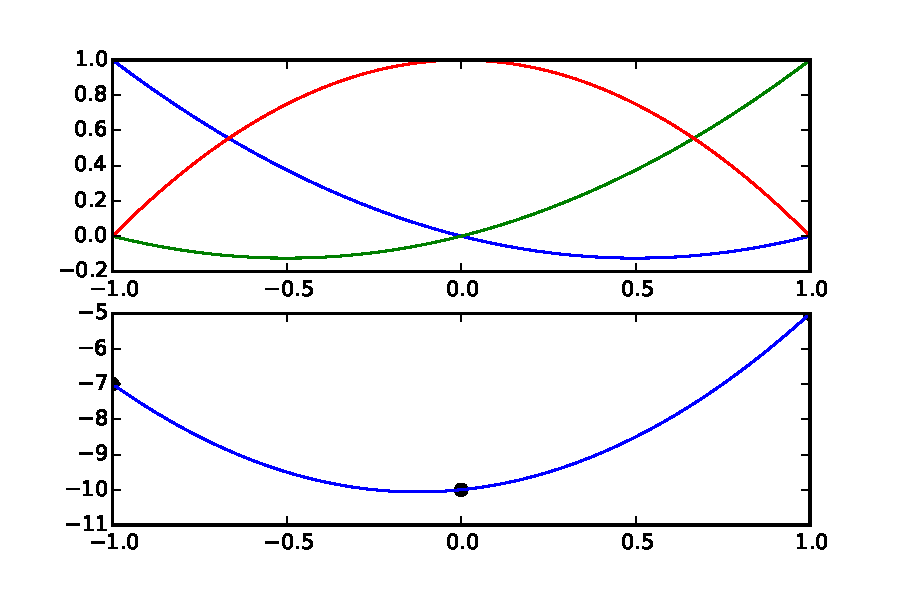
\includegraphics[width=16cm]{func.pdf}
\caption{Interpolating polynomials and the resulting interpolating function}
\label{fig:pols}
\end{figure}

\subsection*{Extension to 2D domains}
Assume we are now interested in conducting interpolation of a function over a spatial 2-dimensional domain where every point is specified by a position vector of the form $\vec x = x\hat i + y\hat j$. We want to know, via interpolation, the value of a function $f(\vec x)$ at an arbitrary point $\vec x$ provided we know the set of n-points $\left\{ {({{\vec x}^1},{f^1}),...,({{\vec x}^n},{f^n})} \right\}$.


\begin{figure}[H]
\centering
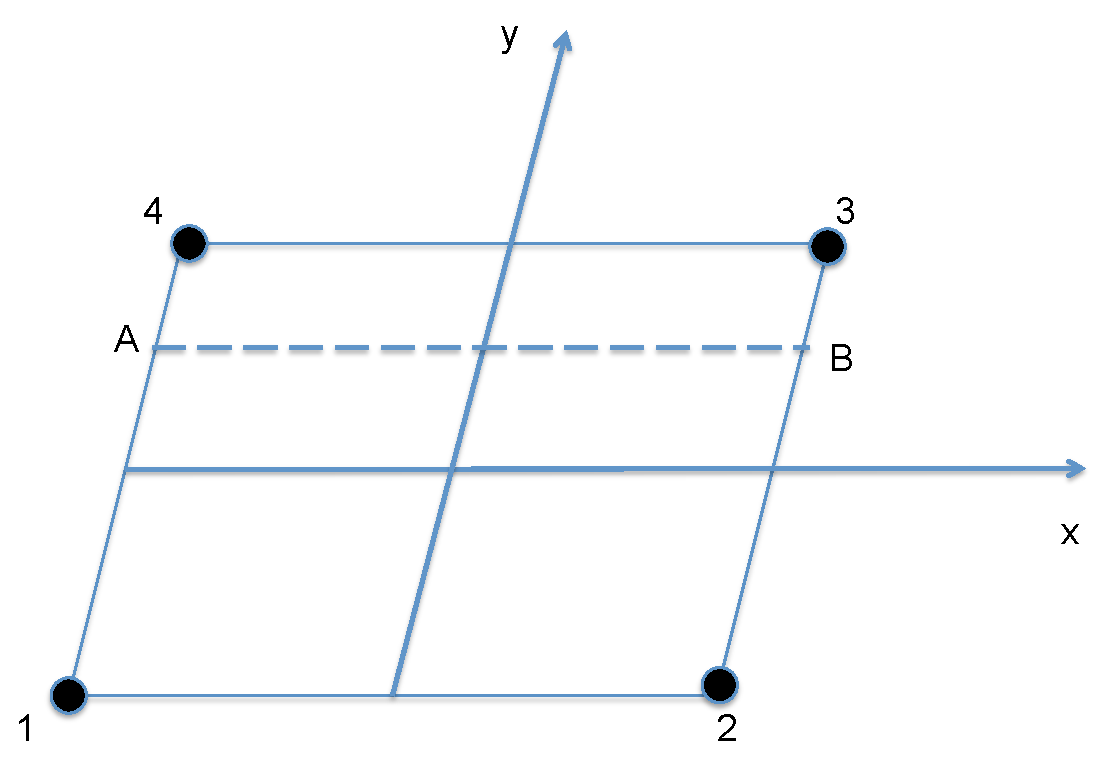
\includegraphics[width=10cm]{element.pdf}
\caption{Basic square domain}
\label{fig:element}
\end{figure}

We first fix $x = {x^A}$ and conduct 1-dimensional interpolation along the $y$ direction as discussed in the previous section as follows (see \cref{fig:onedimn});

\[f({x^A},y) = {L^1}(y){f^1} + {L^4}(y){f^4}\]

\begin{figure}[H]
\centering
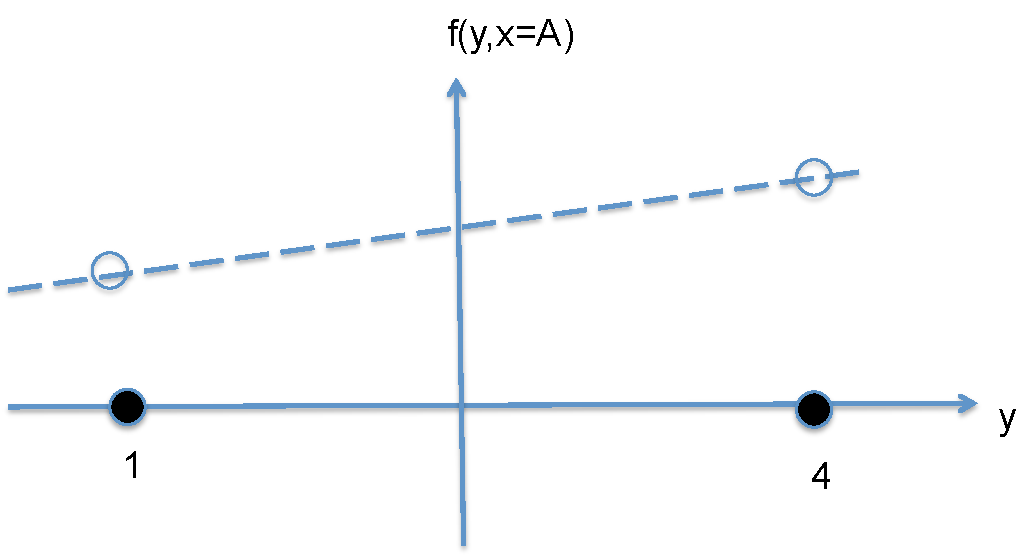
\includegraphics[width=10cm]{inter1D.pdf}
\caption{Interpolation along the $y$-direction}
\label{fig:onedimn}
\end{figure}

Similarly, we can fix $x = {x^B}$ and interpolate once again along the $y$ direction;

\[f({x^B},y) = {L^2}(y){f^2} + {L^3}(y){f^3}.\]

We now conduct the interpolation along the $x$-direction using the functions $f({x^A},y)$ and $f({x^B},y)$ respectively as follows;

\[f(x,y) = {L^A}(x){f({x^A},y)} + {L^B}(x){f({x^B},y)}.\]
\[f(x,y) = {L^A}(x)\left\{ {{L^1}(y){f^1} + {L^4}(y)f{}^4} \right\} + {L^B}(x)\left\{ {{L^2}(y){f^2} + {L^3}(y)f{}^3} \right\}\]
\[f(x,y) = {L^A}(x){L^1}(y){f^1} + {L^A}(x){L^4}(y)f{}^4 + {L^B}(x){L^2}(y){f^2} + {L^B}(x){L^3}(y)f{}^3\]


\begin{align*}
{L^A}(x) & \equiv {L^1}(\xi ) \\
{L^B}(x) & \equiv {L^2}(\xi ) \\
{L^1}(y) & \equiv {L^1}(\xi ) \\
{L^2}(y) & \equiv {L^1}(\xi ) \\
{L^3}(y) & \equiv {L^2}(\xi ) \\
{L^4}(y) & \equiv {L^2}(\xi )
\end{align*}

\[f(x,y) = {N^1}(x,y){f^1} + {N^2}(x,y){f^2} + {N^3}(x,y){f^3} + {N^4}(x,y){f^4}\]

\begin{align*}
{N^1}(x,y) & = {L^1}(x){L^1}(y) \\
{N^2}(x,y) & = {L^2}(x){L^1}(y) \\
{N^3}(x,y) & = {L^2}(x){L^2}(y) \\
{N^4}(x,y) & = {L^1}(x){L^2}(y)
\end{align*}

See Figure \ref{fig:four-nodes-interp} for the shape functions of a 4-nodes element.
\begin{figure}[H]
\centering
	\begin{subfigure}[b]{0.45\textwidth}\qquad
		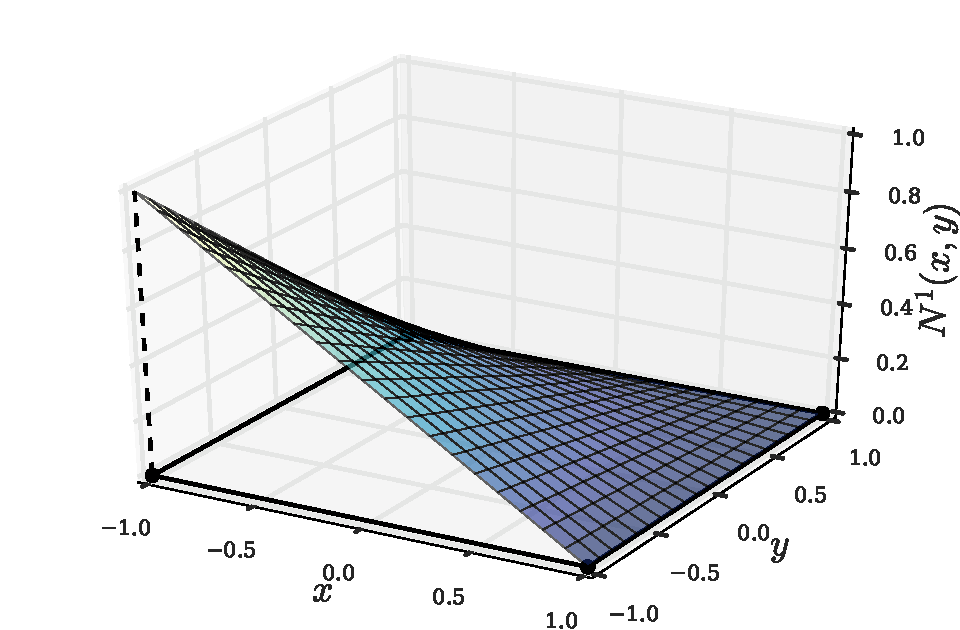
\includegraphics[width=\textwidth]{shape_func-4-nodes-1.pdf}
		\caption{Shape function ${N^1(x,y)=\frac{1}{4}(1-x)(1-y)}$. }
	\end{subfigure}\,
%
	\begin{subfigure}[b]{0.45\textwidth}\qquad
		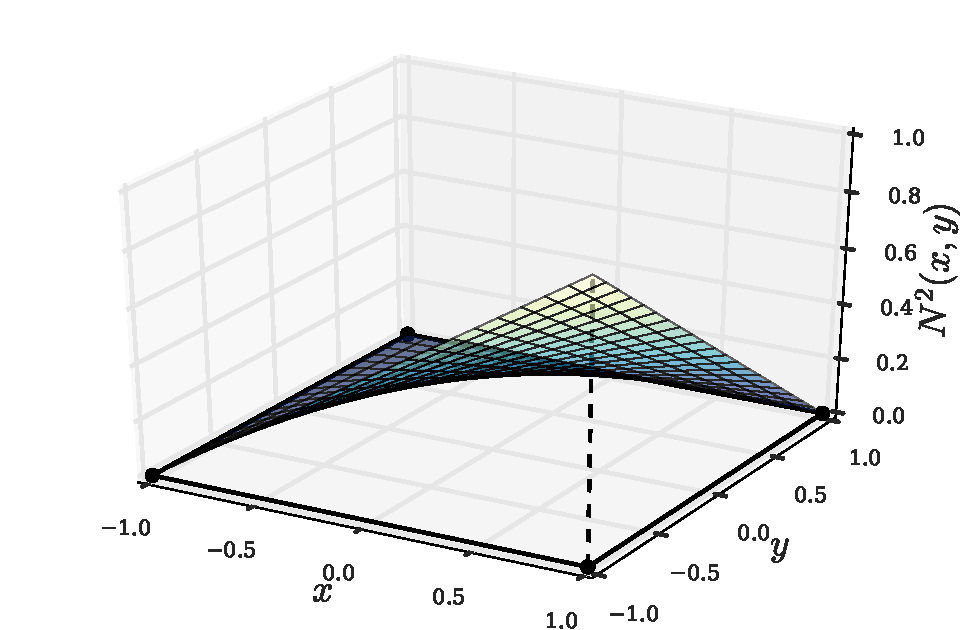
\includegraphics[width=\textwidth]{shape_func-4-nodes-2.pdf}
		\caption{Shape function ${N^2(x,y)=\frac{1}{4}(1+x)(1-y)}$.}
	\end{subfigure}\\
%
	\begin{subfigure}[b]{0.45\textwidth}\qquad
		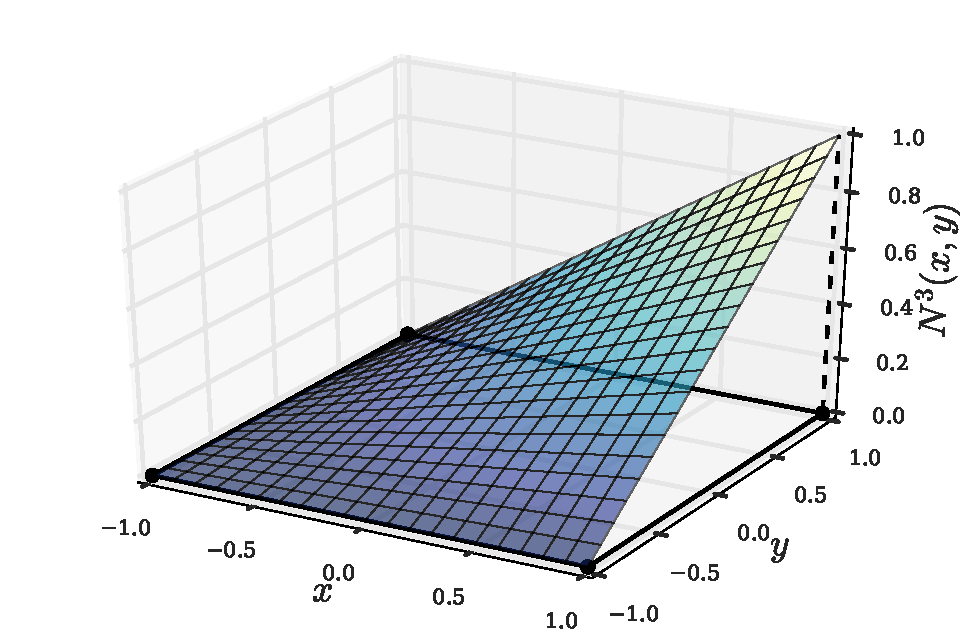
\includegraphics[width=\textwidth]{shape_func-4-nodes-3.pdf}
		\caption{Shape function ${N^3(x,y)=\frac{1}{4}(1+x)(1+y)}$.}
	\end{subfigure}\,
%
	\begin{subfigure}[b]{0.45\textwidth}\qquad
		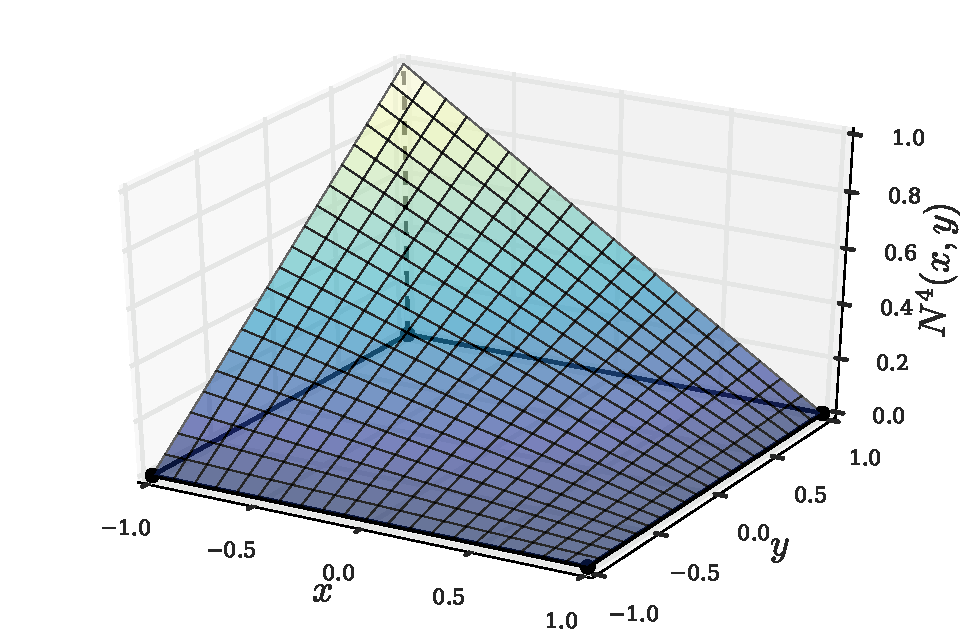
\includegraphics[width=\textwidth]{shape_func-4-nodes-4.pdf}
		\caption{Shape function ${N^4(x,y)=\frac{1}{4}(1-x)(1+y)}$.}
	\end{subfigure}
\caption{Shape functions for a 4-nodes element.}
\label{fig:four-nodes-interp}
\end{figure}

See Figure \ref{fig:nine-nodes-interp} for the shape functions of a 9-nodes element.
\begin{figure}[H]
\centering
	\begin{subfigure}[b]{0.45\textwidth}\qquad
		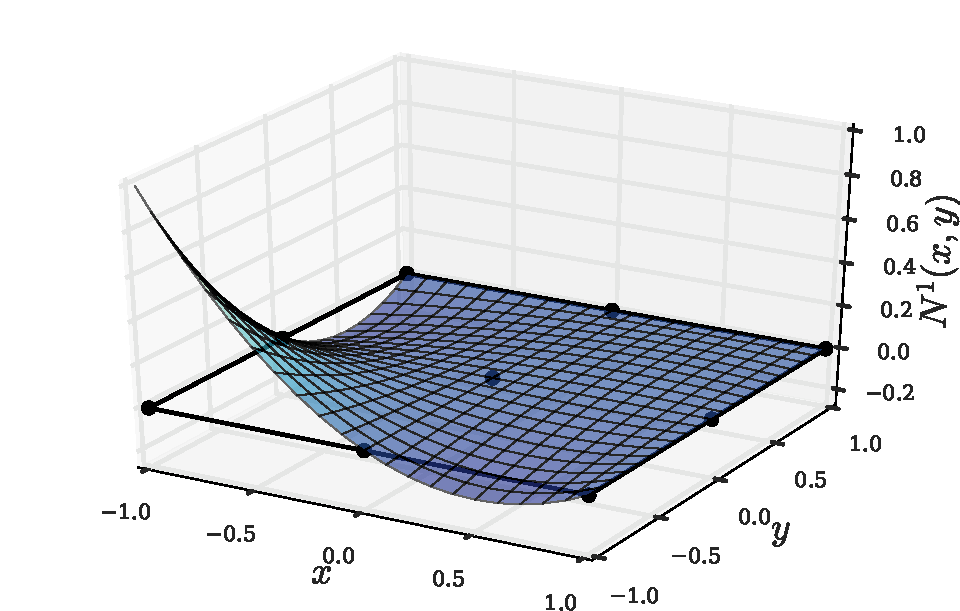
\includegraphics[width=\textwidth]{shape_func-9-nodes-1.pdf}
		\caption{Shape function $N^1(x,y)$. }
	\end{subfigure}\,
%
	\begin{subfigure}[b]{0.45\textwidth}\qquad
		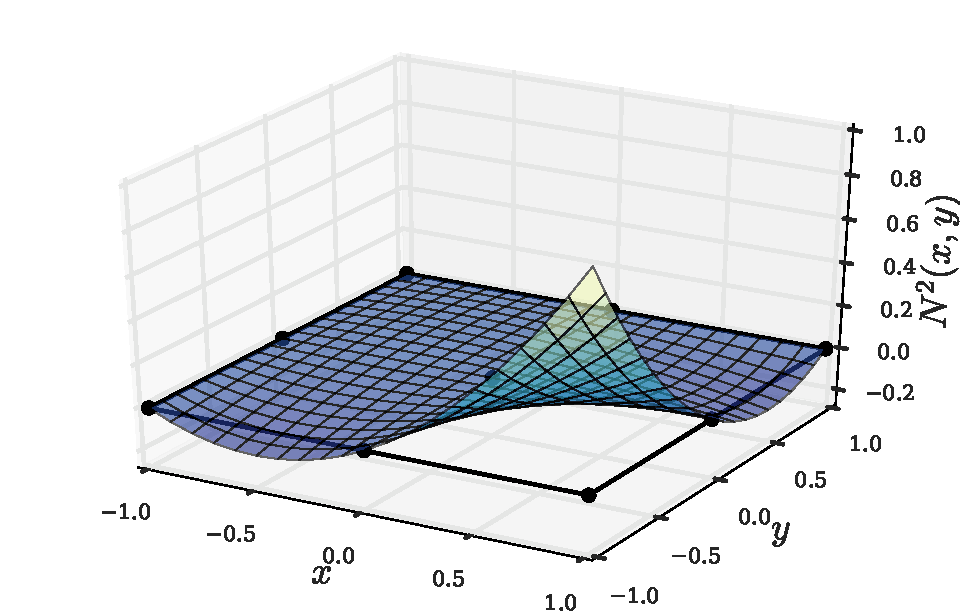
\includegraphics[width=\textwidth]{shape_func-9-nodes-2.pdf}
		\caption{Shape function $N^2(x,y)$.}
	\end{subfigure}\\
%
	\begin{subfigure}[b]{0.45\textwidth}\qquad
		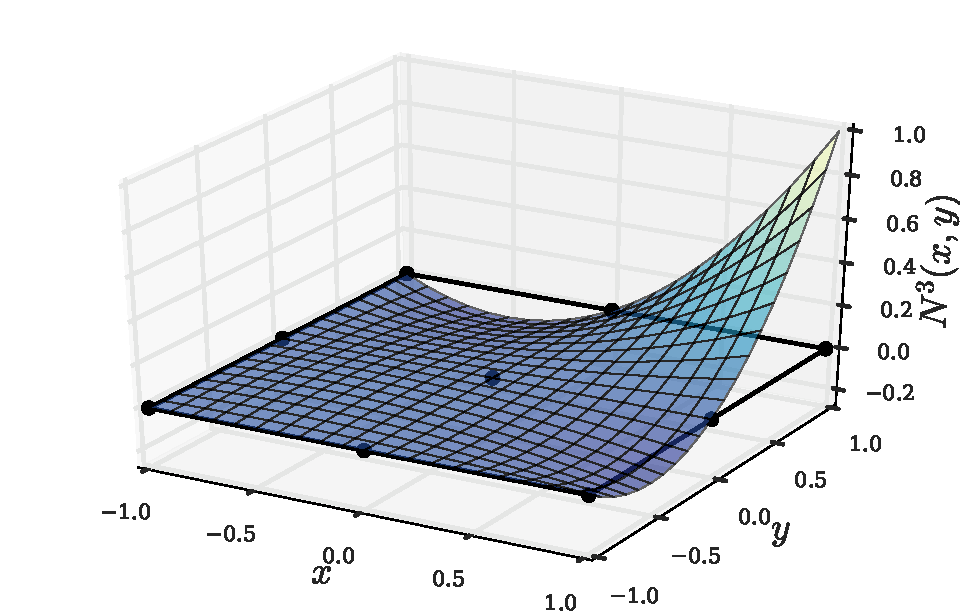
\includegraphics[width=\textwidth]{shape_func-9-nodes-3.pdf}
		\caption{Shape function $N^3(x,y)$.}
	\end{subfigure}\,
%
	\begin{subfigure}[b]{0.45\textwidth}\qquad
		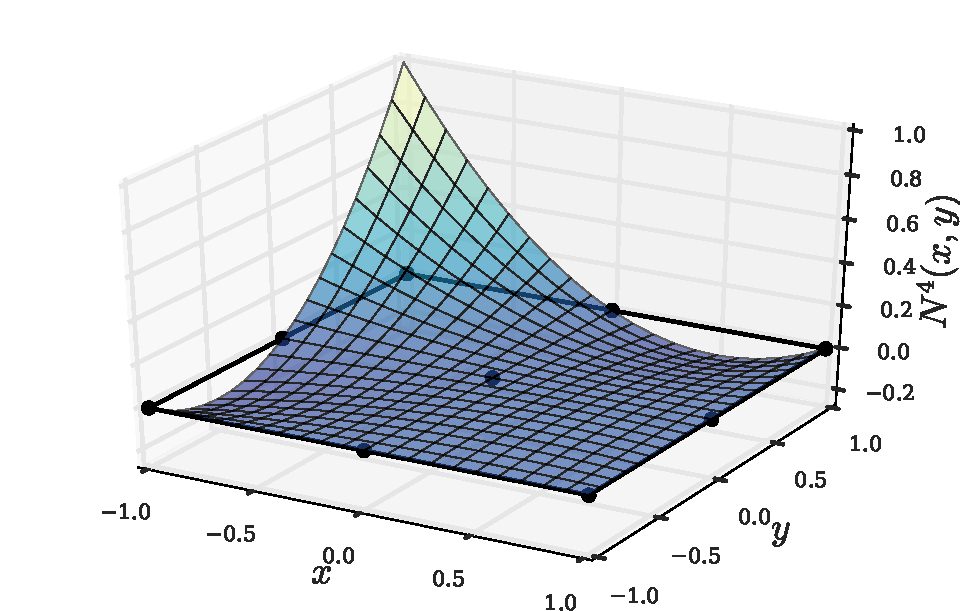
\includegraphics[width=\textwidth]{shape_func-9-nodes-4.pdf}
		\caption{Shape function $N^4(x,y)$.}
	\end{subfigure}\\
	%
	\begin{subfigure}[b]{0.45\textwidth}\qquad
		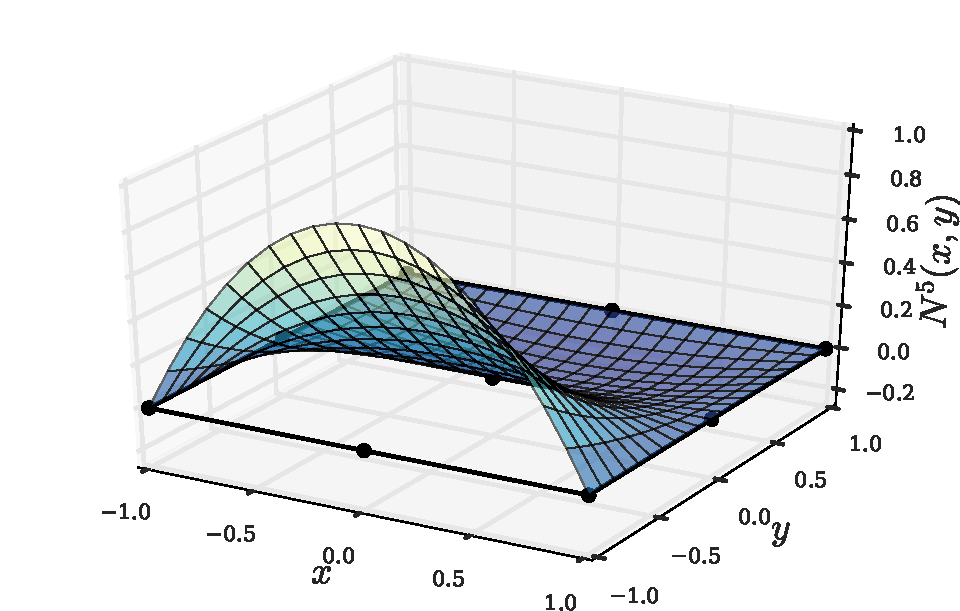
\includegraphics[width=\textwidth]{shape_func-9-nodes-5.pdf}
		\caption{Shape function $N^5(x,y)$.}
	\end{subfigure}\,
%
	\begin{subfigure}[b]{0.45\textwidth}\qquad
		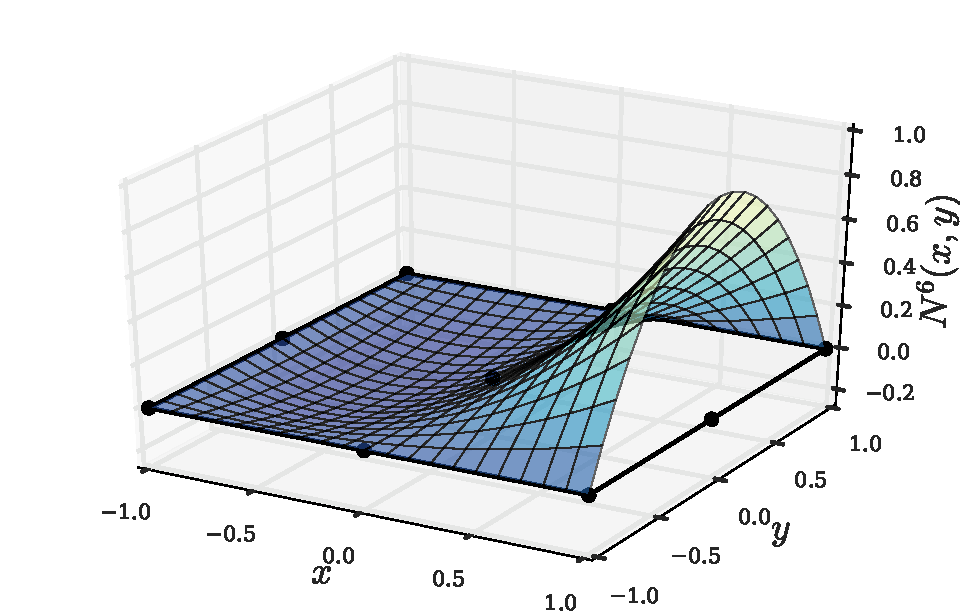
\includegraphics[width=\textwidth]{shape_func-9-nodes-6.pdf}
		\caption{Shape function $N^6(x,y)$.}
	\end{subfigure}
	\caption{Shape functions for a 9-nodes element.}
\end{figure}

\begin{figure}
	\ContinuedFloat
	\centering
	\begin{subfigure}[b]{0.45\textwidth}\qquad
		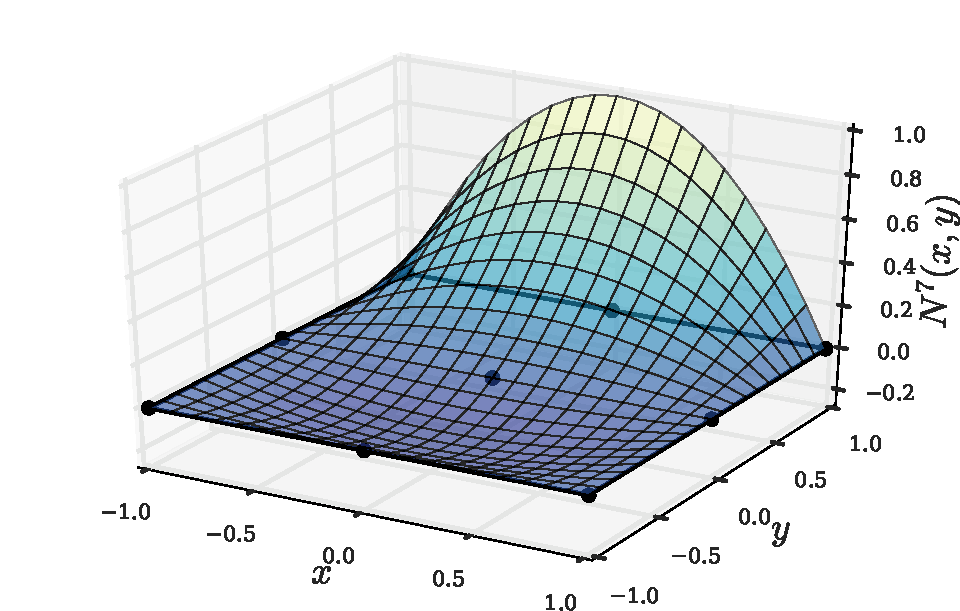
\includegraphics[width=\textwidth]{shape_func-9-nodes-7.pdf}
		\caption{Shape function $N^7(x,y)$.}
	\end{subfigure}\,
%
	\begin{subfigure}[b]{0.45\textwidth}\qquad
		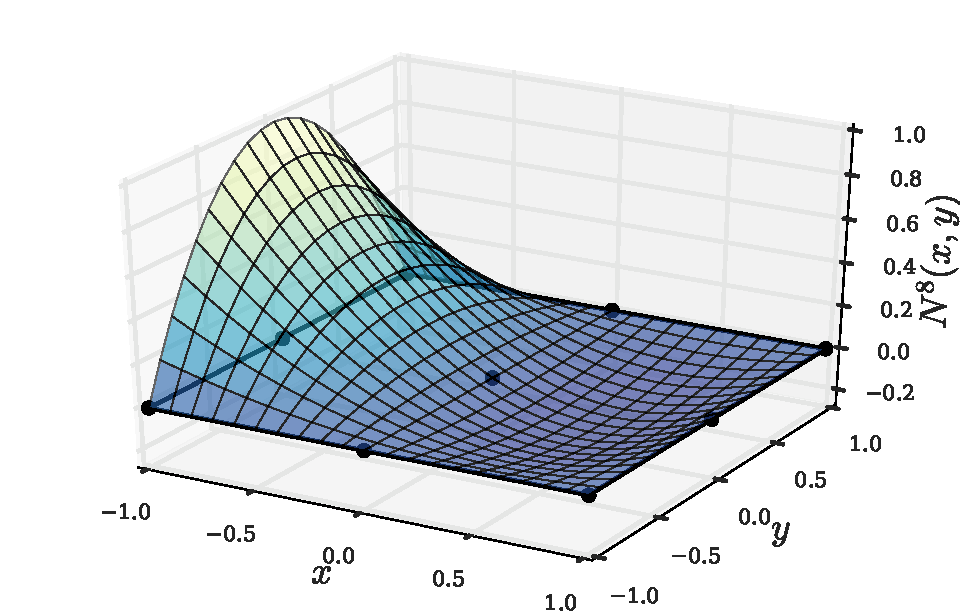
\includegraphics[width=\textwidth]{shape_func-9-nodes-8.pdf}
		\caption{Shape function $N^8(x,y)$.}
	\end{subfigure}\\
	%
	\begin{subfigure}[b]{0.45\textwidth}\qquad
		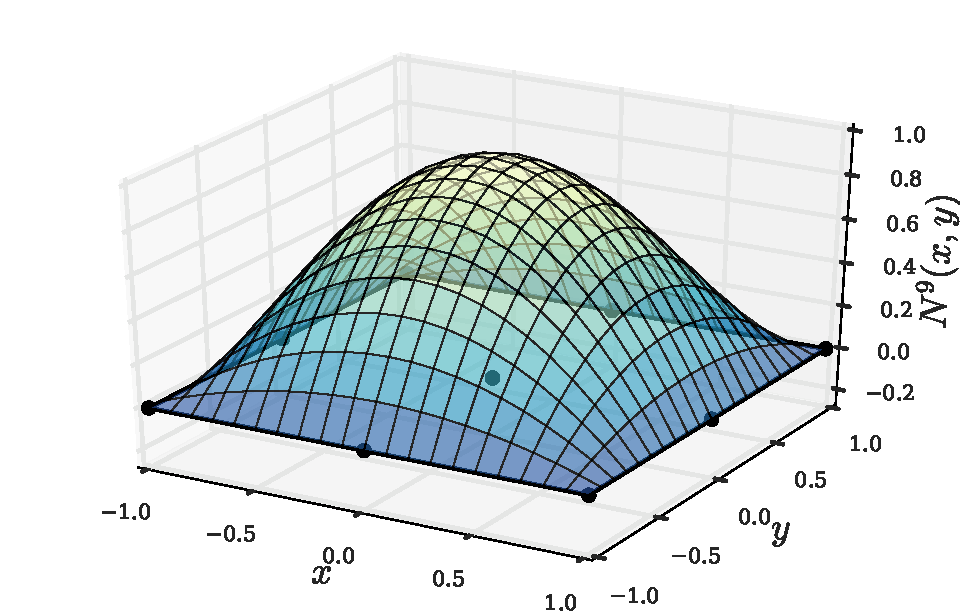
\includegraphics[width=\textwidth]{shape_func-9-nodes-9.pdf}
		\caption{Shape function $N^9(x,y)$.}
	\end{subfigure}
\caption{Shape functions for a 9-nodes element.}
\label{fig:nine-nodes-interp}
\end{figure}

\subsection{Formulation of the finite element matrices}
We now discretize the principle of virtual work repeated below for completeness:

\begin{equation} \label{pvw_2}
\intL_V \sigma_{ij} \delta u_{i,j} dV - \intL_V f_i \delta u_i dV - \intL_{S_t} t_i^n \delta u_i dS = 0.
\end{equation}

For that purpose we will divide the complete domain $V$ into $N$-finite non-overlapping sub-domains over each one of which we will approximate the solution in terms of local interpolating functions. Since the PVW (or weak form of the BVP) has been cast into an integral representation, it is possible to build the total integral considering the contribution of the $N$-sub-domains as follows;

\begin{equation}\label{pvw_dis}
\sum_{e=1}^{NEL} \intL_{V^e} \sigma_{ij} \delta u_{i,j} d{V^e} - \intL_V f_i \delta u_i d{V^e} - \intL_{S_t} t_i^n \delta u_id{S^e} = 0 
\end{equation}

For easiness consider a single sub-domain
\begin{equation} \label{pvw_sing}
\intL_V \sigma_{ij} \delta u_{i,j} dV - \intL_V f_i\delta u_idV - \intL_{S_t} t_i^n \delta u_i dS = 0.
\end{equation}

The involved functions (e.g., displacements, strain, stresses) will be approximated via interpolation of the solution over a determined number of points termed in what follows nodes. Assume for instance that over element $e$ containing $n$ such nodes we know the displacements vector $u_i$. Furthermore, let the displacements for the $p$-node $u^P=[u^P, v^P, w^P]$. Using ideas from interpolation theory it is now possible to approximate the displacements vector over an arbitrary point $\vb{x}$ inside the element as follows
\[u_i(\vb x) = N_i^1(\vb x)u^1 + N_i^2(\vb x)u^2 + \cdots + N_i^P(\vb x)u^P + \cdots + N_i^n(\vb x)u^n\]
or in more general form
\begin{equation} \label{bas_interpol}
{u_i}(\vb x) = N_i^Q(\vb x){u^Q}
\end{equation}

and where the caption superscripts indicate summation over the number of nodes of the element while the subscript refers to the physical character of the variable being interpolated.

\begin{align*}
&\varepsilon_{ij}(\vb x) = B_{ij}^Q(\vb x){u^Q}\\
&\varepsilon_{ij}(\vb x) = \frac{1}{2}( u_{i,j} + u_{j,i} )\\
&\varepsilon_{ij}(\vb x) = \frac{1}{2}\left(\pdv{N_i^Q}{x_j} + \pdv{N_j^Q}{x_i} \right){u^Q}\\
&B_{ij}^Q = \frac{1}{2}\left(\pdv{N_i^Q}{x_j} + \pdv{N_j^Q}{x_i} \right)\\
&\delta {u_i} = N_i^Q(\vb x)\delta {u^Q}\\
&\intL_V C_{ijkl} B_{kl}^P u^P B_{ij}^Q\delta u^Q \dd{V} - \intL_V f_i N_i^Q\delta {u^Q}\dd{V}  - \intL_{S_t} t_i^n N_i^Q\delta {u^Q} \dd{S} = 0\\
&\delta {u^Q}\intL_V B_{ij}^Q C_{ijkl} B_{kl}^P\dd{V}{u^P} - \delta {u^Q}\intL_V N_i^Q{f_i}\dd{V}  - \delta {u^Q}\intL_{S_t} N_i^Qt_i^n\dd{S} = 0 \\
&\delta u^Q f_\sigma ^Q - \delta {u^Q}f_V^Q - \delta u^Q f_c^Q = 0\\
&f_\sigma ^Q - f_V^Q - f_c^Q = 0\\
&f_\sigma ^Q = \intL_V B_{ij}^Q C_{ijkl} B_{kl}^P\dd{V} u^P \equiv K^{QP} u^P\\
&f_V^Q = \intL_V N_i^Q f_i\dd{V} \\
&f_c^Q = \intL_{S_t} N_i^Qt_i^n \dd{S} \\
&K^{QP} u^P = f_V^Q + f_c^Q
\end{align*}

\subsubsection{Formulation in the physical space}
\subsubsection{Formulation in the natural space: the continuum mechanics analogy}
In typical finite element equilibrium equations we need to perform integration over the reference element domain $V_0(\vb{x})$ corresponding to originally arbitrarily shaped sub-domains as created during the meshing process.  In order to proceed with this integration it is useful to consider the following continuum mechanics analogy.

First assume that the actual physical domain $V_0(\vb{x})$ is the result of a deformation process imparted upon the natural domain as shown in \cref{fig:natural domain}. In this analogy, the physical domain $V_0(\vb{x})$ is regarded like a ``deformed'' configuration at an imaginary time $t=t$, while the natural ``undeformed'' domain $V(\vb{r})$   is treated like a reference undeformed configurations at time $t=0$. Both configurations are assumed to be connected through a deformation process;


\begin{equation}
\begin{aligned}
\vb{X}&=\vb{X}(\vb{r})\\
\vb{r}&=\vb{r}(\vb{X})
\end{aligned}
\label{eq:motion}
\end{equation}

\begin{figure}[h]
\centering
\includegraphics[width=8cm]{figure1.pdf}
\caption{Definition of the natural domain}
\label{fig:natural domain}
\end{figure}

 

In \cref{eq:motion} we can understand $\vb{r}$ like a material (Lagrangian) variable and $\vb{X}$ like a spatial (or Eulerian) variable. Using the continuum mechanics analogy it is clear that the ``deformation'' process at the continuum level is fully characterized by the ``deformation'' gradient or Jacobian of the transformation \cref{eq:motion} and defined according to;

\begin{equation}
dX_i=\dfrac{\partial X_i}{\partial r_J}dr_J\equiv J_{iJ}dr_{J}
\label{eq:gradient}
\end{equation}

where $dr_{J}$ and $dX_i$ represent material vectors in the original and deformed configuration. From \cref{eq:gradient} it is evident that the Jacobian contains all the information describing the change of the physical sub-domain with respect to the natural element. For the element integration process we will assume that every element $V(\vb{r})$ in the natural domain deforms into the physical element $V_0(\vb{X})$, thus allowing us to write typical terms like the ones in the material stiffness matrix
\begin{equation}
\intL_{V(\vb{X})} \hat{B}_{ij}^K(\vb{X}) C_{ijkl} \hat{B}_{kl}^P(\vb{X}) dV(\vb{X})\equiv \intL_{V_0(\vb{r})} \hat{B}_{ij}^K(\vb{r}) C_{ijkl} \hat{B}_{kl}^P(\vb{r})J dV_0(\vb{r})
\label{eq:matmatrix}
\end{equation}
where we have used $dV(\vb{X})=JdV(\vb{r})$, with $J$ being the determinant of the deformation gradient and in general we transform functions between the natural and physical space making use of \cref{eq:motion} according to
\begin{equation}
f(\vb{r})=F[\vb{X}(\vb{r})]
\label{eq:funtrans}
\end{equation}


\subsubsection*{Interpolation scheme}
Having identified the fact that the integration process will take place in the natural domain, we will approach the interpolation process directly in this natural space. In the case of the displacement based finite element method all the involved variables will then be obtained via interpolation of nodal displacements. For instance, assume that a given problem variable is defined in the physical space by the tensor $\Phi_{ik...p}(\vb{X})$. The interpolated variable is then written like;

\begin{equation}
\Phi_{ij...p}(\vb{X})=H_{ij...p}^K(\vb{r})\hat{u}^K
\label{eq:interpol}
\end{equation}

where $\hat{u}^K$ represents a vector of nodal points displacements, see \cref{fig:interpol nat dom}, and $H_{ij...p}^K(\vb{r})$ is an interpolator which keeps the tensorial character of the original physical variable $\Phi_{ik...p}(\vb{X})$ and where the super-index makes reference to a nodal identifier (with the summation convention in place).


\begin{figure}[h]
\centering
\includegraphics[width=4cm]{figure2.pdf}
\caption{General interpolation strategy in the natural domain}
\label{fig:interpol nat dom}
\end{figure}
 


Since the primary variable corresponds to displacements it must be kept in mind that $H_{ij...p}^K(\vb{r})$ corresponds to combinations of derivatives (or other arbitrary combinations) of the basic element shape functions defined in;


\begin{equation}
u_i(\vb{X})=N_i^K(\vb{r})\hat{u}^K
\label{eq:el interpol}
\end{equation}



For the general interpolation process we need two kinds of transformations.  First we need to transform integrals over the physical space into integrals into the natural space which corresponds to
\begin{equation}
\intL_{V(\vb{X})} F(\vb{X})dV(\vb{X})\equiv \intL_{V_0(\vb{r})} f(\vb{r})J dV_0(\vb{r})
\label{gen trans}
\end{equation}



Second we need to relate spatial differentiation in both, the physical and spatial domains.  Let us define these operators like $\nabla_i^X$ and $\nabla_I^r$ respectively. It then follows from \cref{eq:funtrans} that
\begin{equation}
\dfrac{\partial F}{\partial X_i}=\dfrac{\partial f}{\partial r_J}\dfrac{\partial r_J}{\partial X_i}
\label{eq:chain}
\end{equation}
from where we can establish the connection between the two operators like


\begin{equation}
\nabla_i^X=J_{iJ}^{-1}\nabla_J^r
\label{eq:fundamental}
\end{equation}


\subsubsection*{The fundamental interpolator}
We further define the fundamental interpolator giving rise to gradients of the primary displacement variable in the physical space according to
\begin{equation}
u_{i,j}(\vb{X})=L_{ij}^K(\vb{r})\hat{u}^K
\label{eq:fund operator}
\end{equation}


This fundamental interpolator  $L_{ik}^K(\vb{r})$ is derived after using \cref{eq:el interpol} and \cref{eq:fundamental} in the physical displacement gradient definition as shown next
\begin{align*}
u_{i,j}(\vb{X})&=\nabla_j^X u_i(\vb{X})\\
u_{i,j}(\vb{X})&=\nabla_j^X N_i^K(\vb{r})\hat{u}^K\\
u_{i,j}(\vb{X})&=J_{jQ}^{-1}\nabla_Q^r N_i^K(\vb{r})\hat{u}^K\\
u_{i,j}(\vb{X})&=J_{jQ}^{-1}N_{i,Q}^K(\vb{r})\hat{u}^K
\end{align*}
then
\begin{equation}
L_{ij}^K(\vb{r})=J_{jQ}^{-1}N_{i,Q}^K(\vb{r})
\label{eq:fundamental interpolator}
\end{equation}

\subsubsection*{Elemental stiffness matrix}
The elemental material stiffness matrix computed in the natural domain of \cref{fig:Nat domain} reads

\begin{equation}
K^{KP}=\intL_{V_0(\vb{r})} \hat{B}_{ij}^K(\vb{r}) C_{ijkl} \hat{B}_{kl}^P(\vb{r})J dV_0(\vb{r})\equiv \intL_{r=-1}^{r=+1}\intL_{s=-1}^{s=+1} \hat{B}_{ij}^K(r,s) C_{ijkl} \hat{B}_{kl}^P(r,s)J(r,s) \mathrm{d}r\mathrm{d}s
\label{eq:elematrix}
\end{equation}



\begin{figure}[h]
\centering
\includegraphics[width=6cm]{figure3.pdf}
\caption{Natural domain of integration}
\label{fig:Nat domain}
\end{figure}
 

Once the interpolator $\hat{B}_{ij}^K(\vb{r})$ has been identified the elemental stiffness matrix is obtained via numerical integration (quadrature) as described in \eqref{eq:eleintegration}

\begin{equation}
\intL_{r=-1}^{r=+1}\intL_{s=-1}^{s=+1} \hat{B}_{ij}^K(r,s) C_{ijkl} \hat{B}_{kl}^P(r,s)J(r,s) \mathrm{d}r\mathrm{d}s\approx \sum_{i,j=1}^\text{NGPTS} \alpha_i \alpha_j \hat{B}_{kl}^K(r_i,s_j)C_{ijkl} \hat{B}_{kl}^P(r_i,s_j) J(r_i,s_j)
\label{eq:eleintegration}
\end{equation}


and where NGPTS corresponds to the number of integration points, $\alpha_j$ is a weighting factor and $r_i,s_j$   are the coordinates of a typical point $\vb{r}$ in the natural space of \cref{fig:Nat domain}.

 
\begin{figure}[h]
\centering
\includegraphics[width=6cm]{figure4.pdf}
\caption{Natural integration domain showing quadrature evaluation nodes}
\label{fig:integration domain}
\end{figure}	 


One important aspect of the numerical integration that has to be kept in mind is accuracy.  Depending on the particularly selected integration scheme, the number of introduced integration points fixes the maximum polynomial order of the considered functions that can be integrated accurately.  In the case of the integrand in \cref{eq:eleintegration}, it is clear that this order increases as the distortion of the physical element  with respect to the natural element increases.  One way of dealing with this dependency of accuracy with element distortion is to make use of adaptative integration techniques which are numerically expensive.  What is actually done in standard FEM analysis is to choose the number of quadrature points beforehand and introduce distortion related error criteria inside the code in such a way that some sort of validation is performed before the numerical integration process is started.

\subsubsection*{Strain displacement interpolator for the infinitesimal strain tensor}
The $Q$-th nodal contribution to the infinitesimal strain-displacement interpolator can be obtained in explicit form as follows. Let $L_x^Q$ and $L_y^Q$ be the spatial differential operators in $x$ and $y$ respectively. We have after expanding \cref{eq:fundamental interpolator}
%
\begin{align*}
L_x^Q & = J_{xP}^{-1}\frac{\partial N^Q}{\partial r_P} \equiv J_{xr}^{-1}\frac{\partial N^Q}{\partial r} + J_{xs}^{-1}\frac{\partial N^Q}{\partial s}\\
L_y^Q & = J_{yP}^{-1}\frac{\partial N^Q}{\partial r_P} \equiv J_{yr}^{-1}\frac{\partial N^Q}{\partial r} + J_{ys}^{-1}\frac{\partial N^Q}{\partial s}
\end{align*}
%
or in matrix form
%
\begin{equation}
\begin{Bmatrix}
L_x^Q\\
L_y^Q
\end{Bmatrix} = 
\begin{bmatrix}
J_{xP}^{-1} &J_{xs}^{- 1}\\
J_{yr}^{-1} &J_{ys}^{- 1}
\end{bmatrix}
\begin{Bmatrix}
\frac{\partial N^Q}{\partial r}\\
\frac{\partial N^Q}{\partial s}
\end{Bmatrix}
\end{equation}

The $Q$-th nodal contribution is then assembled as follows;


\begin{equation}
\begin{Bmatrix}
\pdv{u}{x}\\
\pdv{v}{y}\\
\pdv{u}{y} + \pdv{v}{x}
\end{Bmatrix} =
\begin{bmatrix}
 &L_x^Q &0 \\
\cdots &0 &L_y^Q &\cdots\\
 &L_y^Q &L_{xy}^Q
\end{bmatrix}
\begin{Bmatrix}
\vdots\\
u^Q\\
v^Q\\
\vdots
\end{Bmatrix}
\label{eq:strain inter}
\end{equation}

\begin{algorithm}[H]
\SetAlgoLined
\KwData{Nodal coordinates $x^Q$}
\KwResult{Strain-displacement interpolator $B_{ij}^Q$ }
Compute Jacobian ${J_{iJ}} = \pdv{N_i^Q}{r_J}{\hat x}^Q$\\
Invert Jacobian  ${J_{iJ}} \to J_{iJ}^{ - 1}$\\
Compute fundamental interpolator $L_{ij}^Q = J_{jP}^{ - 1}\pdv{N_i^Q}{r_P}$\\
Assemble $B_{ij}^Q = \frac{1}{2}\left( {L_{ij}^Q + L_{ji}^Q} \right)$ 
\caption{Strain-displacement interpolator}
\end{algorithm}




%Chapter "Wave in Freq domain"

\chapter{Wave propagation problems in the frequency domain}

\section{Problem formulation}

\section{Discretization in complex algebra}

\section{Discretization in real algebra}

\section{Scattering by a micropolar solid}

\section{Coupling with the BEM}

%Chapter "Wave propagation"
%

\chapter{Wave propagation problems in the time domain}

\section{Problem formulation}

\section{Explicit time integration algorithm}

\section{Statement of the Problem}
Consider the discrete dynamic equilibrium equations at time $t$

\begin{equation}
M^{t}A+C^{t}V+K^{t}U=^{t}F
\label{equil}
\end{equation}

where $M$, $C$, $K$ are the assembled mass, damping and stiffness matrix respectively and similarly $^{t}A$, $^{t}V$, $^{t}U$, $^{t}F$ are the nodal accelerations, velocities, displacements and external loads vectors at time $t$. In terms of forces, \cref{equil} can be written like;

\begin{equation}
^{t}F^I+^{t}F^D+^{t}F^s=^{t}F
\label{force equil}
\end{equation}

where $^{t}F^I$, $^{t}F^D$ and $^{t}F^s$ are inertial, damping and elastic nodal forces respectively.

Expanding the acceleration and velocity terms at time $t$ in a consistent finite central differences scheme we have;

\begin{equation}
\begin{aligned}
^{t}A&=\dfrac{1}{\Delta t^2}\left(^{t-\Delta t}U-2^{t}U+^{t+\Delta t}U\right)\\
^{t}V&=\dfrac{1}{2\Delta t}\left(-^{t-\Delta t}U+^{t+\Delta t}U\right)
\end{aligned}
\label{finitediff}
\end{equation}

It is convenient to write \cref{finitediff} like;

\begin{equation}
\begin{aligned}
{}^tA & = {}^t\hat A + \frac{1}{{\Delta {t^2}}}{}^{t + \Delta t}U\\
{}^tV & = {}^t\hat V + \frac{1}{{2\Delta t}}{}^{t + \Delta t}U
\end{aligned}
\label{precorr}
\end{equation}

where:

\begin{equation}
\begin{aligned}
{}^t\hat A & = \frac{1}{{\Delta {t^2}}}\left( {{}^{t - \Delta t}U - 2{}^tU} \right)\\
{}^t\hat V & =  - \frac{1}{{2\Delta t}}{}^{t - \Delta t}U
\end{aligned}
\label{pred}
\end{equation}

are termed predictors, while $\frac{1}{{\Delta {t^2}}}{}^{t + \Delta t}U$ and $\frac{1}{{2\Delta t}}{}^{t + \Delta t}U$ are termed correctors.

Using \cref{finitediff} in \cref{equil} yields;


\begin{equation}
\left(\dfrac{1}{\Delta t^2}M+\dfrac{1}{2\Delta t}C\right) ^{t+\Delta t}U=^{t}F-M{}^t\hat A - C{}^t\hat V - K{}^tU
\label{resequil}
\end{equation}

or after letting;

\[\hat K = \frac{1}{{\Delta {t^2}}}M + \frac{1}{{2\Delta t}}C\]

and

\[{}^t\hat F = {}^tF - M{}^t\hat A - C{}^t\hat V - K{}^tU\] we have;

\[\hat K{}^{t + \Delta t}U = {}^t\hat P\]

which can be solved for ${}^{t + \Delta t}U$.

\begin{algorithm}[H]
\SetAlgoLined
\KwData{Values at $t=0$, Geometry, Material Paramters}
\KwResult{Displacements, Velocity and Acceleration at any time $t=t$ }
Compute predictors ${}^t\hat A$, ${}^t\hat V$, ${}^t\hat U$\\
Assemble  $\hat K$, ${}^t\hat P$\\
Solve $\hat K{}^{t + \Delta t}U = {}^t\hat P$\\
Perform Corrections ${}^tA \leftarrow {}^t\hat A + \frac{1}{{2\Delta {t^2}}}{}^{t + \Delta t}U$ and ${}^tV \leftarrow {}^t\hat V + \frac{1}{{2\Delta t}}{}^{t + \Delta t}U$
\caption{Explicit algorithm}
\end{algorithm}



%%%%%

Redefine forces as follows
\begin{equation}
\begin{aligned}
^{j}F^I&=\dfrac{1}{\Delta t^2}M ^{j}U\\
^{j}F^D&=\dfrac{1}{2 \Delta t}C ^{j}U\\
^{j}F^S&=K ^{j}U
\end{aligned}
\label{redefine}
\end{equation}

and write \eqref{resequil} as;

\begin{equation}
^{t+\Delta t}F^I+^{t+\Delta t}F^D=^{t}F-^{t}F^s+2 ^{t}F^I-^{t-\Delta t}F^I+^{t-\Delta t}F^D
\label{force equil 2}
\end{equation}

\begin{itemize}
\item \eqref{force equil 2} is an equilibrium equation at time $t=t$ allowing to predict the displacements at time $t=t+\Delta t$ in terms of previously known values at times $t$ and $t=t-\Delta t$.

\item The equation is exact within the error introduced by the expansion used in \eqref{finitediff}.

\begin{figure}[h]
\centering
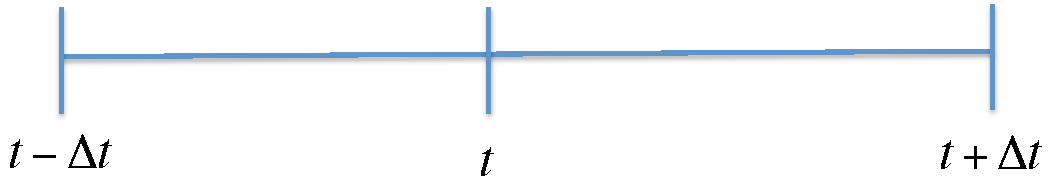
\includegraphics[width=12cm]{img/figure7_0.pdf}
\caption{Definition of the general iteration}
\label{fig:time iteration}
\end{figure}

\item The first predicted solution is at $t=\Delta t$ and we require data at $t=-\Delta t$ and at $t=0$.

\begin{figure}[h]
\centering
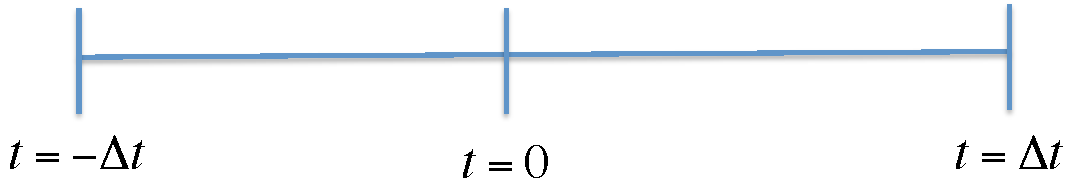
\includegraphics[width=12cm]{img/figure7_1.pdf}
\caption{Definition of the general iteration}
\label{fig:initial time iteration}
\end{figure}

\end{itemize}

\subsection{Damping Assumptions}

\begin{itemize}
\item[1] Use Rayleigh Damping and retain the velocity expansion used in \eqref{finitediff}. That is;

\begin{equation}
C=\alpha M+\beta K
\end{equation}

then we have (in terms of forces);

\begin{equation}
(1+\beta \Delta t^2) ^{t+\Delta t}F^I+\dfrac{\alpha}{2\Delta t} ^{t+\Delta t}F^S=^{t}\hat{F}
\label{Rayleigh}
\end{equation}

where;

\[
^{t}\hat{F}=^{t}R-^{t}F^S+2 ^{t}F^I-^{t-\Delta t}F^I+^{t-\Delta t}F^D
\]

Solution in equation \eqref{Rayleigh} requires the full assembly and factorization of an effective stiffness matrix.

\item[2] Neglect damping (This is however inconvenient for finite domains) 


\begin{equation}
^{t+\Delta t}F^I=^{t}F-^{t}F^S+2 ^{t}F^I-^{t-\Delta t}F^I
\label{Nodamping}
\end{equation}

\item[3] Use Rayleigh damping but modify the velocity expansion introduced in \eqref{finitediff}. Using

\begin{equation}
^{t}V=\dfrac{1}{\Delta t}(^{t}U-^{t-\Delta t}U)
\label{velocity}
\end{equation}

yielding;

\begin{equation}
^{t+\Delta t}F^I=^{t}F-^{t}F^S+2 ^{t}F^{I}-^{t}F^D+^{t-\Delta t}F^D-^{t-\Delta t}F^I
\end{equation}

Defining a set of forces associated to the initial conditions like;

\[
^{t-\Delta t}F^{IC}=^{t-\Delta t}F^I-^{t-\Delta t}F^D
\]

we have

\begin{equation}
^{t+\Delta t}F^I=^{t}F-^{t}F^S+2 ^{t}F^{I}-^{t}F^D-^{t-\Delta t}F^{IC}
\label{modvelocity}
\end{equation}

\end{itemize}

\subsection{Algorithm corresponding to the damping assumption 3}

\begin{figure}[h]
\centering
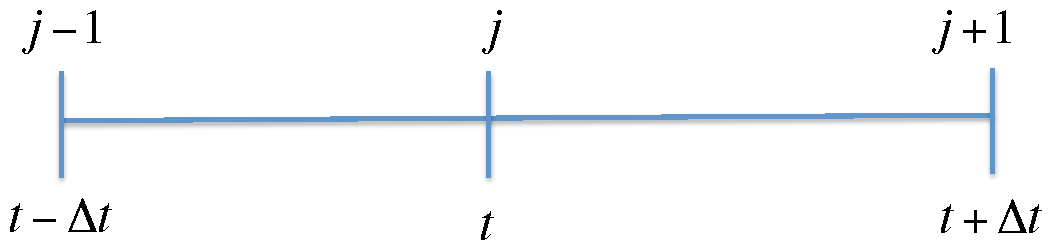
\includegraphics[width=12cm]{img/figure5.pdf}
\caption{Definition of the general iteration}
\label{fig:general iteration}
\end{figure}

Let us write \eqref{modvelocity} like

\begin{equation}
^{j+1}F^I=^{j}F-^{j}F^S+2 ^{j}F^{I}-^{j}F^D-^{j-1}F^{IC}
\label{modveliter}
\end{equation}

where the initialization process corresponds to;


\begin{figure}[h]
\centering
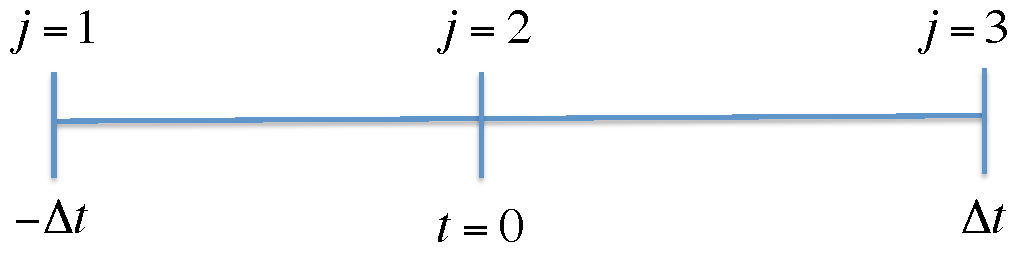
\includegraphics[width=12cm]{img/figure6.pdf}
\caption{Definition of the initial iteration}
\label{fig:initial iteration}
\end{figure}

Applying \eqref{modveliter} for $t=0$ we have;

\[
^{0}F^I=^{0}F-^{0}F^S+2 ^{0}F^{I}-^{0}F^D-^{-\Delta t}F^{IC}
\]

from which it is clear that we require $-^{\Delta t}U$. Applying the central difference expansion at $t=0$ and solving for $-^{\Delta t}U$ yields;

\begin{equation}
^{-\Delta t}U=^{0}F-\Delta t ^{0}V+\dfrac{\Delta t^2}{2} ^{0}A
\label{initialU}
\end{equation}

Using \eqref{initialU} in \eqref{modveliter} allows us to start up the algorithm.

\subsubsection{Particulars}
In what follows we concentrate on this last algorithm and in order to study some details we return to its standard displacements form. Writing \eqref{modveliter} in terms of displacements and re-arranging yields;


\begin{equation}
\dfrac{1}{\Delta t^2}M ^{t+\Delta t}U=^{t}F-(1+\dfrac{\beta}{\Delta t})K ^{t}U+(\dfrac{2}{\Delta t^2}-\dfrac{\alpha}{\Delta t})M ^{t}U-(\dfrac{1}{\Delta t^2} - \dfrac{\alpha}{\Delta t})M ^{t-\Delta t}U+(\dfrac{\beta}{\Delta t}) K ^{t-\Delta t}U
\label{disequil}
\end{equation}

Let;


\[
\begin{aligned}
a_1&=1+\dfrac{\beta}{\Delta t}\\
a_2&=\dfrac{2}{\Delta t^2}-\dfrac{\alpha}{\Delta t}\\
a_3&=\dfrac{1}{\Delta t^2} - \dfrac{\alpha}{\Delta t}\\
a_4&=\dfrac{\beta}{\Delta t}
\end{aligned}
\]


\begin{equation}
^{t+\Delta t}F^I=^{t}F-a_1K ^{t}U+a_2M ^{t}U-a_3M ^{t-\Delta t}U+a_4K ^{t-\Delta t}U
\label{equliassum3}
\end{equation}


\subsection{Decoupling}
Consider the equation for the $i$-th d.o.f;

\begin{equation}
\dfrac{1}{\Delta t^2}M_{ij} ^{t+ \Delta t}U_j=^{t}F_i-a_1K_{ij} ^{t}U_j+a_2M_{ij}^{t}U_j-a_3M_{ij} ^{t-\Delta t}U_j+a_4K_{ij}^{t-\Delta t}U_j
\label{equildecoupled1}
\end{equation}

where we keep $i$ fixed in \eqref{equildecoupled1}. For a lumped mass matrix we can write;

\[
M_{ij}=m_I\delta_{ij}
\]

then \eqref{equildecoupled1} becomes;

\begin{equation}
\dfrac{1}{\Delta t^2}m_I ^{t+ \Delta t}U_i= ^{t}F_I-a_1 K_{ij} ^{t}U_j+a_2 m_I ^{t}U_i-a_3 m_I ^{t-\Delta t} U_i+a_4 K_{ij} ^{t-\Delta t} U_j
\label{equildecoupled2}
\end{equation}

Let;

\begin{equation}
\begin{aligned}
^{t+\Delta t} F_i^I&=\dfrac{1}{\Delta t^2} m_{I} ^{t+\Delta t}U_i\\
^{t} \hat{F}^S_i&=a_1 K_{ij} ^{t}U_j\\
^{t}\hat{F}_i^I&=a_2m_{I} ^{t}U_i\\
^{t-\Delta t}\hat{F}_i^I&=a_3m_{I} ^{t-\Delta t}U_i\\
^{t-\Delta t}\hat{F}_i^S&=a_4K_{ij}^{t-\Delta t}U_j
\end{aligned}
\label{forces2}
\end{equation}

so the recursive equation takes the form;

\begin{equation}
^{t+\Delta t} F_i^I=^{t}F_i-^{t} \hat{F}^S_i+^{t}\hat{F}_i^I-^{t-\Delta t}\hat{F}_i^I+^{t-\Delta t}\hat{F}_i^S
\label{forces3}
\end{equation}

and the algorithm then reduces to;

\begin{algorithm}[H]
\SetAlgoLined
\KwData{Time span, Geometry, Material Paramters}
\KwResult{Displacements, Velocity and Acceleration time histories }
Compute $^{t+\Delta t} F_i^I$\\
Solve for $^{t+\Delta t}U_i=\left(\dfrac{\Delta t^2}{m_I}\right) ^{t+\Delta t}F_{i}^I$\\
Update $^{t}V_i$, $^{t}A_i$
\caption{Summarized Algorithm}
\end{algorithm}

To initialize the algorithm we apply the FD's equations at $t=0$

\[
\dfrac{1}{\Delta t^2}m_I ^{\Delta t}U_i=^{0}F_i-a_1 K_{ij} ^{0}U_j+a_2 m_I ^{0}U_i-a_3 m_I ^{-\Delta t} U_i+a_4 K_{ij} ^{-\Delta t} U_j
\]

where $^{-\Delta t} U_i$ is obtained from \eqref{initialU}

\begin{equation}
^{-\Delta t}U_i=^{0}U_i-\Delta t ^{0}V_i+\dfrac{\Delta t^2}{2} ^{0}A_i
\label{initialU2}
\end{equation}

The initial acceleration is obtained after assuming homogeneous IC's;

\[
m_{I} ^{0}A_i+C_{ij} ^{0}V_j +K_{ij} ^{0}U_j=^{0}F_i
\]

therefore

\[
\begin{aligned}
m_{I} ^{0}A_i=\dfrac{^{0}F_i}{m_I}\\
^{-\Delta t} U_i=\dfrac{\Delta t^2}{2m_I}^{0}F_i
\end{aligned}
\]

Moreover, neglecting the damping effects on the prediction of $^{\Delta t}U_i$ yields;

\[
^{\Delta t} U_i=\dfrac{\Delta t^2}{2m_I}^{0}F_i
\]

\begin{algorithm}[H]
 \SetAlgoLined
 \KwData{Time span, Geometry, Material Paramters}
 \KwResult{Displacements, Velocity and Acceleration time histories }
 Initialize solution vectors ($j=1$)\;
 $^{0}U_i\longrightarrow ^{1}U_i=0$, $^{0}V_i=0$, $^{1}A_i=\dfrac{^{1}R_i}{m_I}$ \;
 Select $\Delta t$ and integration constants $a_1$,$a_2$, $a_3$, $a_4$\;
 Fix 1-st predicted value (let $j=2$)\;
 \[
^{\Delta t} U_i \longleftarrow \dfrac{\Delta t^2}{2m_I} ^{0}F_i\longleftrightarrow \left[^{2}U_i \longleftarrow\dfrac{\Delta t^2}{2m_I} ^{1}F_i \right]
 \]
Time Integration Phase\;
\While{$j \leq N$}{
\[
\begin{aligned}
^{j+1}F^I_i\longleftarrow& ^{j}F_i-a_1 K_{ij} ^{j}U_j+a_2 m_I ^{j}U_j-a_3 m_I ^{j-1} U_i+a_4 K_{ij} ^{j-1} U_j\\
 ^{j+1}U_i\longleftarrow&\dfrac{\Delta t^2}{2m_I} ^{0}F^I_i\\
 ^{j}A_i\longleftarrow&\dfrac{1}{\Delta t^2}\left(^{j-1}U_i-2^{j}U_i+^{j+1}U_i\right)\\
 ^{j}V_i\longleftarrow&\dfrac{1}{2\Delta t}\left(-^{j-1}U_i+^{j+1}U_i\right)\\
 j\longleftarrow&j+1
\end{aligned}
\]
}
\caption{Full Algorithm}
\end{algorithm}

\subsubsection{Nodal Assembler}
In the uncoupled explicit finite element formulation the equation solving process proceeds one degree of freedom at a time. This implies a different assembly process to the one used in an implicit algorithm where a formal coefficient matrix is assembled and inverted. Now the mass, damping and stiffness elemental matrices are used to obtain effective nodal forces at each degree of freedom. In summary the mesh is not covered in an element by element basis, but in a node by node basis. In the following algorithm we discuss this nodal assembly process where in order to solve the displacement at a given degree of freedom prior knowledge of the element contributing to the given node is necessary. In the nodal assembler algorithm the following arrays are needed.

\noindent
ILIST(): Stores the elements connected to the current node.\\
LPLIST():Stores the local position of the current node in each one of the elements of ILIST().\\
NIEL():Number of elements at the current node. This array is used to access ILIST().\\


\begin{algorithm}[H]
\SetAlgoLined
\KwData{Number of nodal points, number of elements, Model}
\KwResult{Displacements, Velocity and Acceleration time histories }
\While {$i \leq NUMNP$}
{
$K\leftarrow NIEL(i)$
%\while {$ik \leq 2$}{
%$jK \leftarrow ID(ik,i)$
%}
}
\caption{Nodal Assembler}
\end{algorithm}
\section{The DRM approach}






%Chapter "Periodic media"
%
\chapter{Periodic media problems}

\section{Bloch analysis}

\section{Implementation}






%Chapter "Computational aspects"
%
\graphicspath{ {./img/COMPU/} }
\chapter{Computational aspects}
\section{Global assembly}
In this section we will discuss the fundamental process of building the system of algebraic equations through the addition or assembly of elemental coefficient matrices as described by \cref{assem} where $K^G$ is the global coefficient matrix; $k^i$ is the local elemental matrix for the $i$-th element; $\assem{i=1}{Numel}$ is the assembly operator and $i$ is an element index ranging betwenn $1$ and the total number of elements $Numel$ that conform the finite element model. Notice that the assembly operator is analogous to the sum operator commonly used in the representation of a series of $N$ terms but it contains information indicating the position of each single term from the element coefficient matrix within the global system. 

\begin{equation}
{K^G}=\assem{i=1}{Numel} k^i.
\label{assem}
\end{equation}

In this section we will describe the fundamental algorithmic steps to perform that process. We first summarize the basic general steps and then illustrate the process through a simple example involving a $2D$ mesh of 4-noded elements. The section is complemented with the python scripts {\bf GLOBAL.py} and the secondary module {\bf assemutil.py}.

\subsection*{The assembly algorithm}
The process of assembly of the elemental coefficient matrices into the global system involves (i) the identification of the active degrees of freedom (or equation numbers) assigned to each node in the mesh (ii) the identification of the relationship between the elemental degrees of freedom and the global degrees of freedom and (iii) the computation of the coefficient matrix for each element in the model.

The first step is easily accomplished by assigning a boundary condition flag to the degrees of freedom existing at each node. Here we use a $0$ value to indicate an active degree of freedom and a $-1$ to indicate a prescribed degree of freedom. This information is stored in a boundary condition array $IBC$, of dimension $nn \times MDIM$, where $nn$ corresponds to the  total number of nodal points and $MDIM$ represents the problem dimensionality. The $IBC$ array is first input by the user and later modified by the program in a process where the boundary condition flag is read and equations are counted and assigned according to the result. If the boundary condition flag is equal to $0$ the program assigns an equation number while it produces a $0$ value if the flag is equal to $-1$.

In the second step the nodes conforming each element are stored in a connectivities array  $IELCON$ of dimension $Numel \times MxNNel$ where $Numel$ is the number of elements in the model and $MxNNel$ is the maximum number of nodes in a given element. Thus each row in the $IELCON$ array stores the nodal point data for the element. Each entry in the $IELCON$ array can now be directly translated into equation numbers using the processed $IBC$ array. This results in the discrete version of the assembly operator $\assem{i=1}{Numel}$ also called the assembly list or the $DME$ operator in our codes.

In the final step the mesh is covered one element at a time and each elemental coefficient matrix is assembled into the global matrix as indicated by the $DME$ operator. The actual computation of the elemental matrix is conducted by an element based subroutine, called here $UEL$, which may be different for each element in the mesh according to different kinematic o material assumptions. The complete process is summarized in \cref{overall} where we describe for completeness additional steps involved in the finite element algorithm. We have introduced aditional global and elemental arrays $RHS^G$ and $rhs^i$ respectively, storing the element nodal excitations and the resulting vector of global excitations. This vector is assembled simultaneously, and using the same data, with the global coefficient matrix. In the final step in the finite element algorithm the system of equations is solved. Notice that the escential boundary conditions were already consideerd during the assembly process and as a result the global algabraic system of equations is ready to be solved. Finally, after the system has been properly solved the nodal results are scattered through the elemnts in a process which is inverse to the assembly operation but that uses the same information contained in the $DME$ operator.\\

\begin{algorithm}[H]
\SetAlgoLined
\KwData{Finite element model}
\KwResult{Field function}
\BlankLine
READ $IBC$ and $IELCON$ arrays ;\\
Compute modified $IBC$ array ;\\
Compute $DME$ operator (using $IBC$ and $IELCON$ arrays);\\
$K^G \leftarrow 0.0$;\\
\BlankLine
\For{$i \leftarrow 1$ to $Numel$}{
    Call UEL(element parameters;$K^i$) ;\\
    $K^G \leftarrow K^G+K^i$ (Assemble each $k^i$ into $K^G$ according to the $DME$ operator);\\
    $RHS^G \leftarrow RHS^G+rhs^i$ (Assemble each $rhs^i$ into $RHS^G$);\\	
	\BlankLine
	}
\BlankLine
Solve ${K^G}{U^G} = RH{S^G}$;\\
Scatter solution to the elements
\caption{Summarized algorithm for the finite element method}
\label{overall}
\end{algorithm}
\newpage
\subsection*{Sample problem}
Consider the mesh shown in \cref{fig:quad}. The problem parameters in this case are $nn=9$, $Numel=4$ and $MxNNel=4$.

\begin{figure}[h]
\centering
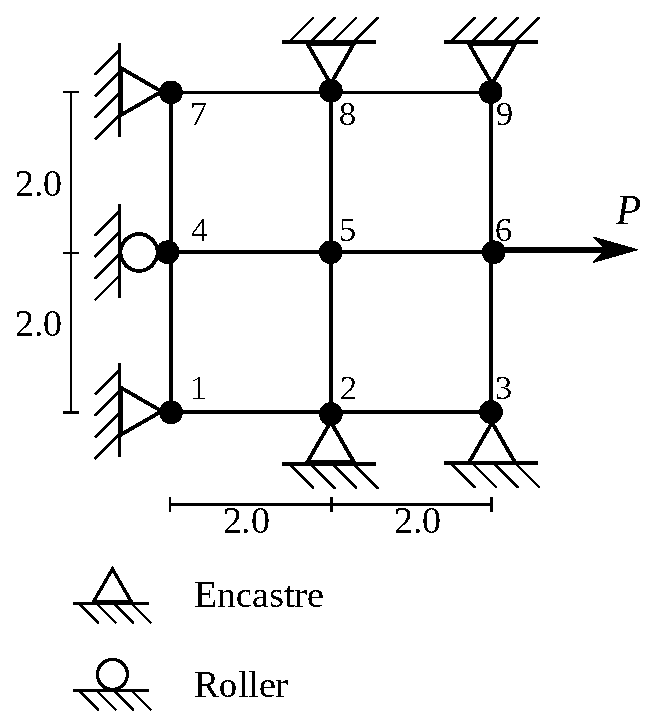
\includegraphics[width=0.75\textwidth]{mesh2.pdf}
\caption{Finite element mesh of 4-noded elements. The global matrix can be assembled using the python scripts {\bf GLOBAL.py} and the secondary module {\bf assemutil.py}. The input files required to run the script are called {\bf nodes.txt} and {\bf eles.txt}}
\label{fig:quad}
\end{figure}
%%

%
The array of boundary conditions as input from the user corresponds to;


\[IBC = \left[ {\begin{array}{*{20}{c}}
{ - 1}&{ - 1}\\
{ - 1}&{ - 1}\\
{ - 1}&{ - 1}\\
{ - 1}&0\\
0&0\\
0&0\\
{ - 1}&{ - 1}\\
{ - 1}&{ - 1}\\
{ - 1}&{ - 1}
\end{array}} \right]\]

while its code-modified version reads;

\[IBC = \left[ {\begin{array}{*{20}{c}}
0&0\\
0&0\\
0&0\\
0&1\\
2&3\\
4&5\\
0&0\\
0&0\\
0&0
\end{array}} \right]\]


Notice that the program changes each $-1$ entry to a $0$ valued entry and assigns an equation number to the position containing an original $0$ entry during an equation-assigning and equation-counting operation. Similarly, the element connectivities for the current example read;

\[IELCON = \left[ {\begin{array}{*{20}{c}}
1&2&5&4\\
2&3&6&5\\
4&5&8&7\\
5&6&9&8
\end{array}} \right]\]

The so-called $DME$ operator is actually the same $IELCON$ but translated into equation numbers for each element. Accordingly in the current example we have;


\[DME = \left[ {\begin{array}{*{20}{c}}
0&0&0&0&2&3&0&1\\
0&0&0&0&4&5&2&3\\
0&1&2&3&0&0&0&0\\
2&3&4&5&0&0&0&0
\end{array}} \right]\]

The definition of the element connectivities and its subsequent translation into degrees of freedom is carried out according to a local element definition like the one shown in \cref{fig:locdof}

\begin{figure}[H]
\centering
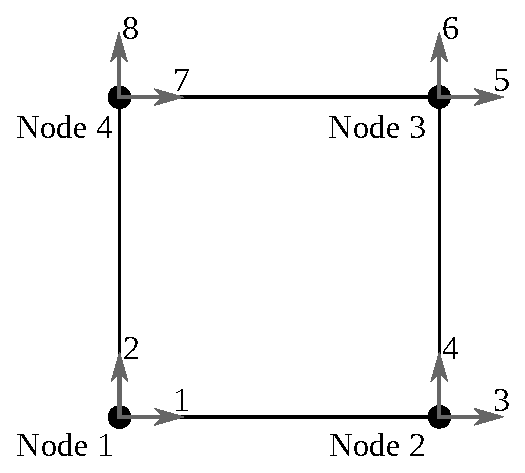
\includegraphics[width=0.50\textwidth]{localdof.pdf}
\caption{Local definition for a 4-noded element.}
\label{fig:locdof}
\end{figure}

As a result the $(i,j)$ entry in the $DME$ corresponds to the global equation number associated with the local degree of freedom $j$ of the $i$ element. For instance the value of $4$ stored at position $(2,5)$ in the current $DME$ indicates that the global equation $4$ corresponds to the local equation $5$ (column index) in element $2$ (row index).\\

The assembly process is then conducetd by identifying the relation between the entries in each row of the $DME$ operator and the list of local degrees of freedom for the reference element shown in \cref{fig:locdof}. Accordingly, for element 2 it follows that the assembly of row $5$ of the local stiffness matrix proceeds as follows;

\begin{align*}
K_{4,4}^G & \leftarrow  K_{4,4}^G + k_{5,5}^2 \\
K_{4,5}^G & \leftarrow  K_{4,5}^G + k_{5,6}^2 \\
K_{4,3}^G & \leftarrow  K_{4,3}^G + k_{5,8}^2
\end{align*}

In \cref{overall} it must be noticed that the local stiffness matrix for each $i$ element is obtained by the call to the local element subroutine $UEL$. In the script GLOBAL.py these elemental routines produce a fictitious matrix filled out with ones and the actual computation of the elemental coefficient amtrix is discussed later.
\section{Python implementations}
\section{Commercial codes and user subroutines}






%Capitulo "Elastodinamica"
%
\chapter{Nonlineal Equilibrium Equations in a Finite Element Discretization}

\section{General Form}


\subsection{Newton-Raphson Scheme}


\section{Algorithm}

%
%%Capitulo "Elastodinamica"
%
\chapter{Equilibrium Equations}

\section{General Equilibrium Equations}
In this section we develop the incremental equations needed in a general non-linear problem.  First, geometric non-linearities valid for any stress-strain pair are considered.  Second, focus is shifted towards the particular case of the Second Piola-Kirchoff-Green Lagrange Strain pair.

Let   represent the current (deformed) configuration of a deformable medium with equilibrium equations and boundary conditions

\begin{equation}
{\sigma _{ij,j}} + {f_i} = 0	 
\end{equation}			

\begin{equation}
{t_i} = {\sigma _{ij}}{\hat n_j}
\end{equation}	 		

where   represents the Cauchy definition of stress (or force per unit of deformed surface) and   the corresponding tractions vector at a surface with outward normal  .  In the equilibrium equations stated in (1) the domain   is unknown which makes the problem inherently non-linear.  On the other hand this equilibrium statement is mathematically indeterminate since 9 unknown stress components must be solved out of 6 field equations.  The indeterminacy is destroyed after the problem is kinematically described and connected to the stress field via constitutive modeling which can involve additional sources of non-linearity.  To summarize the problem is non-linear since the domain   is unknown, this is what we typically call a Geometric Non-linearity and will be reflected in the mathematical description of changes in configuration.



\subsection{Lagrangian description of the equilibrium equations}
The conceptual definition of Cauchy stress is the only one useful for the engineer since it describes forces per unit deformed surface.  This validity is clearly identified in the fact that the equilibrium equations stated in (1) have been formulated in the stressed deformed domain   where the body is in fact in equilibrium.  The difficulty associated with the unknown domain may be dealt with in alternative ways.  In the case of a solid body it is convenient to refer everything to the undeformed or reference configuration (with known domain)   and proceed from there using linearization which corresponds to a Total Lagrangian (TL) approach.  It is then useful to understand the transformation of the problem to   via pullback operations.  This process implies the introduction or consideration of mathematically  defined stress definitions and newly developed kinematic descriptions.  In this section we consider such transformations first from a dynamic point of view and later using thermodynamic principles we address the problem of identifying the proper strain measures.
\begin{figure}[h]
\centering
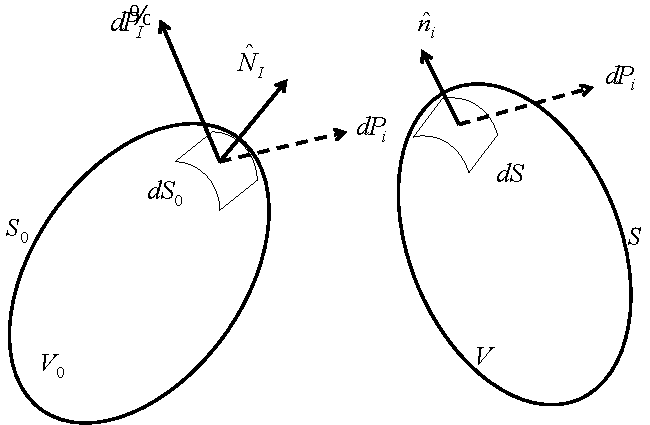
\includegraphics[width=8cm]{img/figure1_2.pdf}
\caption{Definition of the natural domain}
\label{fig:natural domain}
\end{figure}

\subsubsection*{Nanson's formula}
For the treatment that follows it will result useful to consider the relation between oriented differential surface elements in the reference and deformed configurations in the so-called Nanson's formula;

\begin{equation}
\hat{n}_{i}dS=\frac{\rho}{\rho _0}\hat{N}_I f_{Ii}dS_0
\label{nanson}
\end{equation}

\subsubsection*{Lagrangian stress definition}
Let be the differential force associated to the Cauchy physical stress such

\begin{equation}
d{P_i} = {t_i}dS \equiv {\sigma _{ji}}{n_j}dS
\label{diff stress 1}
\end{equation}	 								(3)

Assume that   can also be obtained in the undeformed configuration associated with a new traction definition;

\begin{equation}
d{P_i} = t_i^0d{S_0} \equiv T_{Ii}^0{N_I}d{S_0} \equiv {\sigma _{ji}}{n_j}dS
\label{diff stress 2}	
\end{equation} 						(4)

Using Nanson's formula it is possible to write;

\begin{equation}
T_{Ii}^0{N_I}d{S_0} \equiv {\sigma _{ji}}\frac{{{\rho _0}}}{\rho }{N_I}{f_{Ij}}d{S_0}
\label{equiv}
\end{equation}	 							(5)

Which simplifies into

\begin{equation}
T_{Ii}^0 = \frac{{{\rho _0}}}{\rho }{f_{Ij}}{\sigma _{ji}}
\label{simplified}
\end{equation}	 									(6)

and this is the asymmetric First Piola-Kirchoff stress tensor.

Assume now that there is a pseudo-force in the undeformed configuration   which results from a pullback operation on the physical force  .  Recalling the kinematic connection between the current and undeformed configurations

\begin{equation}
d{X_I} = {f_{Ii}}d{x_i}
\label{pseudo}
\end{equation}	 									(7)

where   is the inverse deformation gradient, we can write for the force and pseudo-force vectors;

\begin{equation}
d{\tilde P_I} = {f_{Ii}}d{P_i}.
\label{for and psefor}
\end{equation}									(8)

Now we can define a tractions vector   in the undeformed configuration and associated with the pseudo-force   like

\begin{equation}
d{\tilde P_I} = {\tilde t_I}d{S_0} \equiv {T_{JI}}{N_J}d{S_0}
\label{unde tracts 1}
\end{equation}	 								(9)

where we have at the same time introduced the associated stress tensor.  It then directly follows that;

\begin{equation}
{T_{JI}}{N_J}d{S_0} = {f_{Ii}}d{P_i} \equiv {f_{Ii}}{\sigma _{ji}}{n_j}dS
\label{unde tracts 2}	 
\end{equation}							(10)

once again using Nanson's formula we can write

\begin{equation}
{T_{JI}}{N_J}d{S_0} = {f_{Ii}}{\sigma _{ji}}\frac{{{\rho _0}}}{\rho }{N_J}{f_{Jj}}d{S_0}
\label{unde tracts 3}
\end{equation}	 							(11)

and

\begin{equation}
{T_{JI}} = \frac{{{\rho _0}}}{\rho }{f_{Jj}}{\sigma _{ji}}{f_{Ii}}
\label{unde tracts 4}
\end{equation}	 								(12)

which corresponds to the symmetric Second Piola-Kirchoff stress tensor.

For the derivations that follow and in the actual computational implementation it will be convenient to have the inverse relationships expressing the Cauchy stress tensor in terms of the First and Second Piola-Kirchoff stress definitions.

Once again recall that   and use the definition found for the first PK stress tensor to write



\section{Equilibrium in Weak Form}

%%Capitulo "Elastodinamica"
%
\chapter{Nonlinear Problems}

\section{Nonlinear Scalar Equations}


\subsection{Newton-Raphson Scheme}


\section{Systems of Nonlinear Equations}

%%Chapter "Elemental Matrices"
%
\chapter{Elemental Matrices-The Continuum Mechanics Analogy}

\section{Statement of the Problem}
In the incremental equilibrium equations (22) we need to perform integration over the reference element domain $V_0(\vec{x})$ corresponding to originally arbitrarily shaped sub-domains as created during the meshing process.  In order to proceed with this integration it is useful to consider the following continuum mechanics analogy.

First assume that the actual physical domain $V_0(\vec{x})$ is the result of a deformation process imparted upon the natural domain as shown in Figure A1. In this analogy, the physical domain $V_0(\vec{x})$ is regarded like a "deformed" configuration at an imaginary time $t=t$, while the natural "un-deformed" domain $V(\vec{r})$   is treated like a reference un-deformed configurations at time $t=0$. Both configurations are assumed to be connected through a deformation process;


\begin{equation}
\begin{aligned}
\vec{X}&=\vec{X}(\vec{r})\\
\vec{r}&=\vec{r}(\vec{X})
\end{aligned}
\label{motion}
\end{equation}

\begin{figure}[h]
\centering
\includegraphics[width=12cm]{img/figure1.pdf}
\caption{Definition of the natural domain}
\label{fig:natural domain}
\end{figure}

 

In \eqref{motion} we can understand $\vec{r}$ like a material (Lagrangian) variable and $\vec{X}$ like a spatial (or Eulerian) variable. Using the continuum mechanics analogy it is clear that the "deformation" process at the continuum level is fully characterized by the "deformation" gradient or Jacobian of the transformation \eqref{motion} and defined according to;

\begin{equation}
dX_i=\dfrac{\partial X_i}{\partial r_J}dr_J\equiv J_{iJ}dr_J
\label{gradient}
\end{equation}

where $dr_J$ and $dX_i$ represent material vectors in the original and deformed configuration. From \eqref{gradient} it is evident that the Jacobian contains all the information describing the change of the physical sub-domain with respect to the natural element. For the element integration process we will assume that every element $V(\vec{r})$ in the natural domain deforms into the physical element $V_0(\vec{X})$ thus allowing us to write typical terms like the ones in the material stiffness matrix in (22) like;

\begin{equation}
\int\limits_{V_0(\vec{X})} \hat{B}_{ij}^K(\vec{X}) C_{ijkl} \hat{B}_{kl}^P(\vec{X}) dV_0(\vec{X})\equiv \int\limits_{V_0(\vec{X})} \hat{B}_{ij}^K(\vec{r}) C_{ijkl} \hat{B}_{kl}^P(\vec{r})J dV(\vec{r})
\label{matmatrix}
\end{equation}


where we have used $dV(\vec{X})=JdV(\vec{r})$, with $J$ being the determinant of the deformation gradient and in general we transform functions between the natural and physical space making use of \eqref{motion} according to;

\begin{equation}
f(\vec{r})=F[\vec{X}(\vec{r})]
\label{funtrans}
\end{equation}

	 								
\subsubsection{Interpolation scheme}
Having identified the fact that the integration process will take place in the natural domain we will approach the interpolation process directly in this natural space.  In the case of the displacement based finite element method all the involved variables will then be obtained via interpolation of nodal displacements.  For instance, assume that a given problem variable is defined in the physical space by the tensor $\Phi_{ik...p}(\vec{X})$. The interpolated variable is then obtained like;

\begin{equation}
\Phi_{ij...p}(\vec{X})=H_{ij...p}^K(\vec{r})\hat{u}^K
\label{interpol}
\end{equation}	 						

where $\hat{u}^K$ represents a vector of nodal points displacements, see Figure \ref{fig:interpol nat dom}, and $H_{ij...p}^K(\vec{r})$ is an interpolator which keeps the tensorial character of the original physical variable $\Phi_{ik...p}(\vec{X})$   and where the super-index makes reference to a nodal identifier and the summation convention applies.


\begin{figure}[h]
\centering
\includegraphics[width=6cm]{img/figure2.pdf}
\caption{General interpolation strategy in the natural domain}
\label{fig:interpol nat dom}
\end{figure}
 


Since the primary variable corresponds to displacements it must be kept in mind that $H_{ij...p}^K(\vec{r})$ corresponds to combinations of derivatives (or other arbitrary combinations) of the basic element shape functions defined in;


\begin{equation}
u_i(\vec{X})=N_i^K(\vec{r})\hat{u}^K
\label{el interpol}
\end{equation}



For the general interpolation process we need two kinds of transformations.  First we need to transform integrals over the physical space into integrals into the natural space which corresponds to;


\begin{equation}
\int\limits_{V_0(\vec{X})} F(\vec{X})dV_0(\vec{X})\equiv \int\limits_{V_0(\vec{r})} f(\vec{r})J dV(\vec{r})
\label{gen trans}
\end{equation}



Second we need to relate spatial differentiation in both, the physical and spatial domains.  Let us define these operators like $\bigtriangledown_i^X$ and $\bigtriangledown_I^r$ respectively. It then follows from \eqref{funtrans} and the chain rule of differentiation that;

\begin{equation}
\dfrac{\partial F}{\partial X_i}=\dfrac{\partial f}{\partial r_J}\dfrac{\partial r_J}{\partial X_i}
\label{chain}
\end{equation}

from where we can establish the connection between the two operators like


\begin{equation}
\bigtriangledown_i^X=J_{Ji}^{-1}\bigtriangledown_I^r
\label{fundamental}
\end{equation}

We further define the fundamental interpolator giving rise to gradients of the primary displacement variable in the physical space according to;


\begin{equation}
u_{i,j}(\vec{X})=L_{ij}^K(\vec{r})\hat{u}^K
\label{fund operator}
\end{equation}


This fundamental interpolator  $L_{ik}^K(\vec{r})$ is derived after using \eqref{el interpol} and \eqref{fundamental} in the physical displacement gradient definition as shown next;


\[
\begin{aligned}
u_{i,j}(\vec{X})&=\bigtriangledown_j^X u_i(\vec{X})\\
u_{i,j}(\vec{X})&=\bigtriangledown_j^X N_i^K(\vec{r})\hat{u}^K\\
u_{i,j}(\vec{X})&=J_{Qj}^{-1}\bigtriangledown_Q^r N_i^K(\vec{r})\hat{u}^K\\
u_{i,j}(\vec{X})&=J_{Qj}^{-1}N_{i,Q}^K(\vec{r})\hat{u}^K
\end{aligned}
\]

then

\begin{equation}
L_{ij}^K(\vec{r})=J_{Qj}^{-1}N_{i,Q}^K(\vec{r})
\label{fundamental interpolator}
\end{equation}

\subsubsection{Elemental stiffness matrix}
The elemental material stiffness matrix computed in the natural domain of Figure A3 reads;



\begin{equation}
K^{KP}=\int\limits_{V_0(\vec{r})} \hat{B}_{ij}^K(\vec{r}) C_{ijkl} \hat{B}_{kl}^P(\vec{r})J dV(\vec{r})\equiv \int\limits_{r=-1}^{r=+1}\int\limits_{s=-1}^{s=+1} \hat{B}_{ij}^K(r,s) C_{ijkl} \hat{B}_{kl}^P(r,s)J(r,s) \mathrm{d}r\mathrm{d}s
\label{elematrix}
\end{equation}



\begin{figure}[h]
\centering
\includegraphics[width=12cm]{img/figure3.pdf}
\caption{Natural domain of integration}
\label{fig:Nat domain}
\end{figure}	 		
 

Once the interpolator $\hat{B}_{ij}^K(\vec{r})$ has been identified the elemental stiffness matrix is obtained via numerical integration (quadrature) as described in \eqref{elematrix};

\begin{equation}
\int\limits_{r=-1}^{r=+1}\int\limits_{s=-1}^{s=+1} \hat{B}_{ij}^K(r,s) C_{ijkl} \hat{B}_{kl}^P(r,s)J(r,s) \mathrm{d}r\mathrm{d}s\approx \sum_{i,j=1}^{NGPTS} \alpha_i \alpha_j \hat{B}_{kl}^K(r_i,s_j)C_{ijkl} \hat{B}_{kl}^P(r_i,s_j) J(r_i,s_j)
\label{eleinetgration}
\end{equation}

	 													(A13)

and where NGPTS corresponds to the number of integration points, $\alpha_j$ is a weighting factor and $r_i,s_j$   are the coordinates of a typical point $\vec{r}$ in the natural space of Figure A4 .

 
 \begin{figure}[h]
\centering
\includegraphics[width=12cm]{img/figure4.pdf}
\caption{Natural integration domain showing quadrature evaluation nodes}
\label{fig:integration domain}
\end{figure}	 


One important aspect of the numerical integration that has to be kept in mind is accuracy.  Depending on the particularly selected integration scheme, the number of introduced integration points fixes the maximum polynomial order of the considered functions that can be integrated accurately.  In the case of the integrand in \eqref{eleinetgration}, it is clear that this order increases as the distortion of the physical element  with respect to the natural element increases.  One way of dealing with this dependency of accuracy with element distortion is to make use of adaptative integration techniques which are numerically expensive.  What is actually done in standard FEM analysis is to choose the number of quadrature points beforehand and introduce distortion related error criteria inside the code in such a way that some sort of validation is performed before the numerical integration process is started.
%%Chapter "Elemental Matrices"
%
\chapter{Explicit Dynamic Analysis}

\section{Statement of the Problem}
Consider the discrete dynamic equilibrium equations at time $t$

\begin{equation}
M^{t}A+C^{t}V+K^{t}U=^{t}F
\label{equil}
\end{equation}

where $M$, $C$, $K$ are the assembled mass, damping and stiffness matrix respectively and similarly $^{t}A$, $^{t}V$, $^{t}U$, ${t}F$ are the nodal accelerations, velocities, displacements and external loads vectors at time $t$. In terms of forces \eqref{equil} can be written like;

\begin{equation}
^{t}F^I+^{t}F^D+^{t}F^s=^{t}F
\label{force equil}
\end{equation}

where $^{t}F^I$, $^{t}F^D$ and $^{t}F^s$ are inertial, damping and elastic components respectively.

Expanding the acceleration and velocity terms at time $t$ in a consistent finite central differences scheme we have;

\begin{equation}
\begin{aligned}
^{t}A&=\dfrac{1}{\Delta t^2}\left(^{t-\Delta t}U-2^{t}U+^{t+\Delta t}U\right)\\
^{t}V&=\dfrac{1}{2\Delta t}\left(-^{t-\Delta t}U+^{t+\Delta t}U\right)
\end{aligned}
\label{finitediff}
\end{equation}

Using \eqref{finitediff} in \eqref{force equil} yields;


\begin{equation}
\left(\dfrac{1}{\Delta t^2}M+\dfrac{1}{2\Delta t}C\right) ^{t+\Delta t}U=^{t}F-\left(K-\dfrac{2}{\Delta t^2}M\right) ^{t}U-\left(\dfrac{1}{\Delta t^2}M-\dfrac{1}{2\Delta t^2}C\right)^{t-\Delta t}U
\label{resequil}
\end{equation}

Redefine forces as follows
\begin{equation}
\begin{aligned}
^{j}F^I&=\dfrac{1}{\Delta t^2}M ^{j}U\\
^{j}F^D&=\dfrac{1}{2 \Delta t}C ^{j}U\\
^{j}F^S&=K ^{j}U
\end{aligned}
\label{redefine}
\end{equation}

and write \eqref{resequil} as;

\begin{equation}
^{t+\Delta t}F^I+^{t+\Delta t}F^D=^{t}F-^{t}F^s+2 ^{t}F^I-^{t-\Delta t}F^I+^{t-\Delta t}F^D
\label{force equil 2}
\end{equation}

\begin{itemize}
\item \eqref{force equil 2} is an equilibrium equation at time $t=t$ allowing to predict the displacements at time $t=t+\Delta t$ in terms of previously known values at times $t$ and $t=t-\Delta t$.

\item The equation is exact within the error introduced by the expansion used in \eqref{finitediff}.

\begin{figure}[h]
\centering
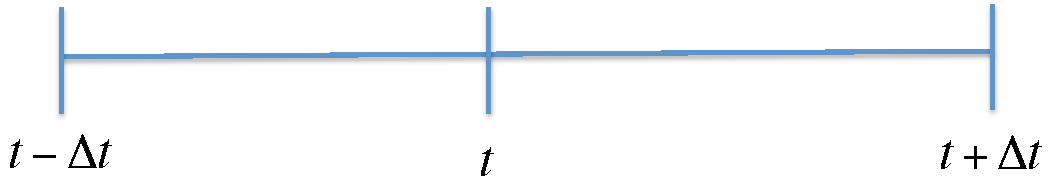
\includegraphics[width=12cm]{img/figure7_0.pdf}
\caption{Definition of the general iteration}
\label{fig:time iteration}
\end{figure}

\item The first predicted solution is at $t=\Delta t$ and we require data at $t=-\Delta t$ and at $t=0$.

\begin{figure}[h]
\centering
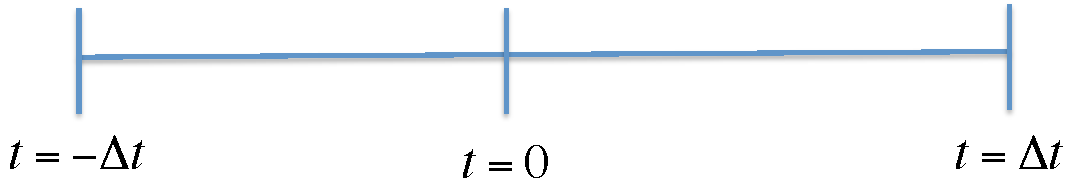
\includegraphics[width=12cm]{img/figure7_1.pdf}
\caption{Definition of the general iteration}
\label{fig:initial time iteration}
\end{figure}

\end{itemize}

\subsection{Damping Assumptions}

\begin{itemize}
\item[1] Use Rayleigh Damping and retain the velocity expansion used in \eqref{finitediff}. That is;

\begin{equation}
C=\alpha M+\beta K
\end{equation}

then we have (in terms of forces);

\begin{equation}
(1+\beta \Delta t^2) ^{t+\Delta t}F^I+\dfrac{\alpha}{2\Delta t} ^{t+\Delta t}F^S=^{t}\hat{F}
\label{Rayleigh}
\end{equation}

where;

\[
^{t}\hat{F}=^{t}R-^{t}F^S+2 ^{t}F^I-^{t-\Delta t}F^I+^{t-\Delta t}F^D
\]

Solution in equation \eqref{Rayleigh} requires the full assembly and factorization of an effective stiffness matrix.

\item[2] Neglect damping (This is however inconvenient for finite domains) 


\begin{equation}
^{t+\Delta t}F^I=^{t}F-^{t}F^S+2 ^{t}F^I-^{t-\Delta t}F^I
\label{Nodamping}
\end{equation}

\item[3] Use Rayleigh damping but modify the velocity expansion introduced in \eqref{finitediff}. Using

\begin{equation}
^{t}V=\dfrac{1}{\Delta t}(^{t}U-^{t-\Delta t}U)
\label{velocity}
\end{equation}

yielding;

\begin{equation}
^{t+\Delta t}F^I=^{t}F-^{t}F^S+2 ^{t}F^{I}-^{t}F^D+^{t-\Delta t}F^D-^{t-\Delta t}F^I
\end{equation}

Defining a set of forces associated to the initial conditions like;

\[
^{t-\Delta t}F^{IC}=^{t-\Delta t}F^I-^{t-\Delta t}F^D
\]

we have

\begin{equation}
^{t+\Delta t}F^I=^{t}F-^{t}F^S+2 ^{t}F^{I}-^{t}F^D-^{t-\Delta t}F^{IC}
\label{modvelocity}
\end{equation}

\end{itemize}

\subsection{Algorithm corresponding to the damping assumption 3}

\begin{figure}[h]
\centering
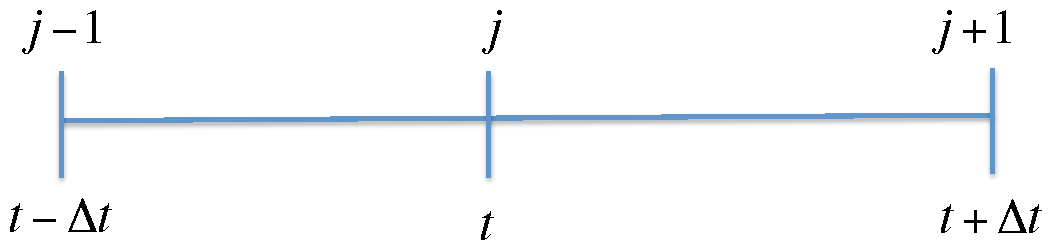
\includegraphics[width=12cm]{img/figure5.pdf}
\caption{Definition of the general iteration}
\label{fig:general iteration}
\end{figure}

Let us write \eqref{modvelocity} like

\begin{equation}
^{j+1}F^I=^{j}F-^{j}F^S+2 ^{j}F^{I}-^{j}F^D-^{j-1}F^{IC}
\label{modveliter}
\end{equation}

where the initialization process corresponds to;


\begin{figure}[h]
\centering
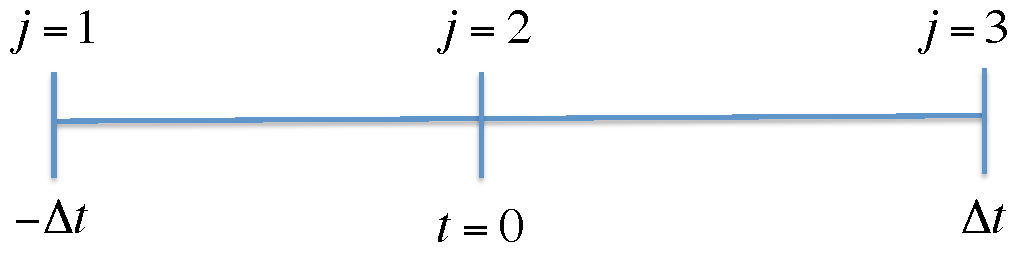
\includegraphics[width=12cm]{img/figure6.pdf}
\caption{Definition of the initial iteration}
\label{fig:initial iteration}
\end{figure}

Applying \eqref{modveliter} for $t=0$ we have;

\[
^{0}F^I=^{0}F-^{0}F^S+2 ^{0}F^{I}-^{0}F^D-^{-\Delta t}F^{IC}
\]

from which it is clear that we require $-^{\Delta t}U$. Applying the central difference expansion at $t=0$ and solving for $-^{\Delta t}U$ yields;

\begin{equation}
^{-\Delta t}U=^{0}F-\Delta t ^{0}V+\dfrac{\Delta t^2}{2} ^{0}A
\label{initialU}
\end{equation}

Using \eqref{initialU} in \eqref{modveliter} allows us to start up the algorithm.

\subsubsection{Particulars}
In what follows we concentrate on this last algorithm and in order to study some details we return to its standard displacements form. Writing \eqref{modveliter} in terms of displacements and re-arranging yields;


\begin{equation}
\dfrac{1}{\Delta t^2}M ^{t+\Delta t}U=^{t}F-(1+\dfrac{\beta}{\Delta t})K ^{t}U+(\dfrac{2}{\Delta t^2}-\dfrac{\alpha}{\Delta t})M ^{t}U-(\dfrac{1}{\Delta t^2} - \dfrac{\alpha}{\Delta t})M ^{t-\Delta t}U+(\dfrac{\beta}{\Delta t}) K ^{t-\Delta t}U
\label{disequil}
\end{equation}

Let;


\[
\begin{aligned}
a_1&=1+\dfrac{\beta}{\Delta t}\\
a_2&=\dfrac{2}{\Delta t^2}-\dfrac{\alpha}{\Delta t}\\
a_3&=\dfrac{1}{\Delta t^2} - \dfrac{\alpha}{\Delta t}\\
a_4&=\dfrac{\beta}{\Delta t}
\end{aligned}
\]


\begin{equation}
^{t+\Delta t}F^I=^{t}F-a_1K ^{t}U+a_2M ^{t}U-a_3M ^{t-\Delta t}U+a_4K ^{t-\Delta t}U
\label{equliassum3}
\end{equation}


\subsection{Decoupling}
Consider the equation for the $i$-th d.o.f;

\begin{equation}
\dfrac{1}{\Delta t^2}M_{ij} ^{t+ \Delta t}U_j=^{t}F_i-a_1K_{ij} ^{t}U_j+a_2M_{ij}^{t}U_j-a_3M_{ij} ^{t-\Delta t}U_j+a_4K_{ij}^{t-\Delta t}U_j
\label{equildecoupled1}
\end{equation}

where we keep $i$ fixed in \eqref{equildecoupled1}. For a lumped mass matrix we can write;

\[
M_{ij}=m_I\delta_{ij}
\]

then \eqref{equildecoupled1} becomes;

\begin{equation}
\dfrac{1}{\Delta t^2}m_I ^{t+ \Delta t}U_i= ^{t}F_I-a_1 K_{ij} ^{t}U_j+a_2 m_I ^{t}U_i-a_3 m_I ^{t-\Delta t} U_i+a_4 K_{ij} ^{t-\Delta t} U_j
\label{equildecoupled2}
\end{equation}

Let;

\begin{equation}
\begin{aligned}
^{t+\Delta t} F_i^I&=\dfrac{1}{\Delta t^2} m_{I} ^{t+\Delta t}U_i\\
^{t} \hat{F}^S_i&=a_1 K_{ij} ^{t}U_j\\
^{t}\hat{F}_i^I&=a_2m_{I} ^{t}U_i\\
^{t-\Delta t}\hat{F}_i^I&=a_3m_{I} ^{t-\Delta t}U_i\\
^{t-\Delta t}\hat{F}_i^S&=a_4K_{ij}^{t-\Delta t}U_j
\end{aligned}
\label{forces2}
\end{equation}

so the recursive equation takes the form;

\begin{equation}
^{t+\Delta t} F_i^I=^{t}F_i-^{t} \hat{F}^S_i+^{t}\hat{F}_i^I-^{t-\Delta t}\hat{F}_i^I+^{t-\Delta t}\hat{F}_i^S
\label{forces3}
\end{equation}

and the algorithm then reduces to;

\begin{algorithm}[H]
\SetAlgoLined
\KwData{Time span, Geometry, Material Paramters}
\KwResult{Displacements, Velocity and Acceleration time histories }
Compute $^{t+\Delta t} F_i^I$\\
Solve for $^{t+\Delta t}U_i=\left(\dfrac{\Delta t^2}{m_I}\right) ^{t+\Delta t}F_{i}^I$\\
Update $^{t}V_i$, $^{t}A_i$
\caption{Summarized Algorithm}
\end{algorithm}

To initialize the algorithm we apply the FD's equations at $t=0$

\[
\dfrac{1}{\Delta t^2}m_I ^{\Delta t}U_i=^{0}F_i-a_1 K_{ij} ^{0}U_j+a_2 m_I ^{0}U_i-a_3 m_I ^{-\Delta t} U_i+a_4 K_{ij} ^{-\Delta t} U_j
\]

where $^{-\Delta t} U_i$ is obtained from \eqref{initialU}

\begin{equation}
^{-\Delta t}U_i=^{0}U_i-\Delta t ^{0}V_i+\dfrac{\Delta t^2}{2} ^{0}A_i
\label{initialU2}
\end{equation}

The initial acceleration is obtained after assuming homogeneous IC's;

\[
m_{I} ^{0}A_i+C_{ij} ^{0}V_j +K_{ij} ^{0}U_j=^{0}F_i
\]

therefore

\[
\begin{aligned}
m_{I} ^{0}A_i=\dfrac{^{0}F_i}{m_I}\\
^{-\Delta t} U_i=\dfrac{\Delta t^2}{2m_I}^{0}F_i
\end{aligned}
\]

Moreover, neglecting the damping effects on the prediction of $^{\Delta t}U_i$ yields;

\[
^{\Delta t} U_i=\dfrac{\Delta t^2}{2m_I}^{0}F_i
\]

\begin{algorithm}[H]
 \SetAlgoLined
 \KwData{Time span, Geometry, Material Paramters}
 \KwResult{Displacements, Velocity and Acceleration time histories }
 Initialize solution vectors ($j=1$)\;
 $^{0}U_i\longrightarrow ^{1}U_i=0$, $^{0}V_i=0$, $^{1}A_i=\dfrac{^{1}R_i}{m_I}$ \;
 Select $\Delta t$ and integration constants $a_1$,$a_2$, $a_3$, $a_4$\;
 Fix 1-st predicted value (let $j=2$)\;
 \[
^{\Delta t} U_i \longleftarrow \dfrac{\Delta t^2}{2m_I} ^{0}F_i\longleftrightarrow \left[^{2}U_i \longleftarrow\dfrac{\Delta t^2}{2m_I} ^{1}F_i \right]
 \]
Time Integration Phase\;
\While{$j \leq N$}{
\[
\begin{aligned}
^{j+1}F^I_i\longleftarrow& ^{j}F_i-a_1 K_{ij} ^{j}U_j+a_2 m_I ^{j}U_j-a_3 m_I ^{j-1} U_i+a_4 K_{ij} ^{j-1} U_j\\
 ^{j+1}U_i\longleftarrow&\dfrac{\Delta t^2}{2m_I} ^{0}F^I_i\\
 ^{j}A_i\longleftarrow&\dfrac{1}{\Delta t^2}\left(^{j-1}U_i-2^{j}U_i+^{j+1}U_i\right)\\
 ^{j}V_i\longleftarrow&\dfrac{1}{2\Delta t}\left(-^{j-1}U_i+^{j+1}U_i\right)\\
 j\longleftarrow&j+1
\end{aligned}
\]
}
\caption{Full Algorithm}
\end{algorithm}

\subsubsection{Nodal Assembler}
In the uncoupled explicit finite element formulation the equation solving process proceeds one degree of freedom at a time. This implies a different assembly process to the one used in an implicit algorithm where a formal coefficient matrix is assembled and inverted. Now the mass, damping and stiffness elemental matrices are used to obtain effective nodal forces at each degree of freedom. In summary the mesh is not covered in an element by element basis, but in a node by node basis. In the following algorithm we discuss this nodal assembly process where in order to solve the displacement at a given degree of freedom prior knowledge of the element contributing to the given node is necessary. In the nodal assembler algorithm the following arrays are needed.

\noindent
ILIST(): Stores the elements connected to the current node.\\
LPLIST():Stores the local position of the current node in each one of the elements of ILIST().\\
NIEL():Number of elements at the current node. This array is used to access ILIST().\\


\begin{algorithm}[H]
\SetAlgoLined
\KwData{Number of nodal points, number of elements, Model}
\KwResult{Displacements, Velocity and Acceleration time histories }
\While {$i \leq NUMNP$}
{
$K\leftarrow NIEL(i)$
%\while {$ik \leq 2$}{
%$jK \leftarrow ID(ik,i)$
%}
}
\caption{Nodal Assembler}
\end{algorithm}







%%%%%%%%%%%%%%%%%%%%%%%%%%%%%%%%%%%%%%%%%%%%%%%%%%%%%%%%%%%%%%%%%%%%%%%%%%%%
%%%%%% Bibliografia %%%%%%%%%%
%%Para referenciar sin cita en el texto
%\nocite{}
\addcontentsline{toc}{chapter}{Referencias}
\bibliographystyle{babunsrt}
%\bibliography{informe}

%%%%%%%%%%%%%%%%%%%%%%%%%%%%%%%%%%%%%%%%%%%%%%%%%%%%%%%%%%%%%%%%%%%%%%%%%%%%

\end{document}

